% IEEE S&P 2027 submission format; requires IEEEtran.cls v1.8b.
\documentclass[conference,compsoc]{IEEEtran}

\usepackage[T1]{fontenc}
\usepackage[utf8]{inputenc}
\usepackage{booktabs}
\usepackage{tabularx}
\usepackage{array}
\usepackage{graphicx}
\usepackage{amsmath}
\usepackage[dvipsnames,table]{xcolor}
\usepackage{tikz}
\usetikzlibrary{arrows.meta,positioning,fit,calc,matrix,shapes.geometric}
\usepackage[hyphens]{url}
\usepackage{hyperref}

\hypersetup{hidelinks,pdfauthor={}}
\newcommand{\scope}{\textsc{Scope}}
\newcommand{\NRR}{\textsf{U}}
\newcommand{\NRA}{\textsf{A}}
\newcommand{\NRV}{\textsf{?}}
\newcommand{\NA}{--}
\newcommand{\evidenceStrong}{\cellcolor{ForestGreen!22}Strong}
\newcommand{\evidenceLimited}{\cellcolor{Goldenrod!24}Limited}
\newcommand{\evidenceNone}{\cellcolor{Gray!18}No verified direct evidence}
\newcommand{\soktakeaway}[2]{%
  \par\smallskip\noindent
  \fcolorbox{MidnightBlue!45}{MidnightBlue!5}{%
    \parbox{\dimexpr\columnwidth-2\fboxsep-2\fboxrule\relax}{%
      \footnotesize\textbf{\color{MidnightBlue!85!black}#1.} #2%
    }%
  }\par\smallskip
}
\newcolumntype{Y}{>{\raggedright\arraybackslash}X}
\newcommand{\auditpartial}{\textbf{P}}
% Additive finite-candidate reconciliation; historical snapshots retained.
\newcommand{\SnapshotN}{60}
\newcommand{\SnapshotCore}{43}
\newcommand{\SnapshotA}{15}
\newcommand{\SnapshotB}{28}
\newcommand{\SnapshotAdjacent}{17}
\newcommand{\FinalN}{82}
\newcommand{\FinalCore}{58}
\newcommand{\FinalAdjacent}{24}


\title{SoK: Transfer Boundaries of LLM and Agent\\Side-Channel Defenses}
\author{}

\begin{document}
\maketitle

\begin{abstract}
Side-channel defenses for LLM serving and agent systems are evaluated at one operating point and then reused at another: a different emitter, tool dispatcher, model or observer. We ask which changes invalidate a measured defense result. Our unit of analysis is the evaluated result record, which binds an outcome to its target, receiver, intervention boundary, attacker fit, workload and cost object. A map of 82 study families, 39 source-bound records and a nine-item reuse audit show that the evidence deployment needs is the evidence least often reported: inference is bound for 17 of 20 mitigation families, but matched adaptation for only 2 of 11 applicable families and utility at the protected operating point for 3 of 17; no family reports an explicit hardware or temporal holdout. Four controlled experiments then exercise each boundary: upstream padding does not protect a re-emitting frontend, idempotent cover does not preserve state, timing exposes cover that length-only evaluation scores at chance, and defense calibration does not transfer as a scalar. Moving a calibrated defense from MiniMax to GLM raises cancellation balanced accuracy from 50.0\% to 70.8\% while lowering return from 67.3\% to 50.0\%: protection is exchanged between targets rather than uniformly degraded. We distill these results into a decision procedure: identify the boundary a deployment changes, require evidence bound on that boundary, and otherwise re-measure it.
\end{abstract}

\section{Introduction}\label{sec:introduction}
Encryption conceals message content, yet LLM engines and agents expose packet sizes, cache timing, visited domains and tool sequences \cite{weiss2024prompt,promptpeek2025,earlybird2025,agentprint2025,uitraces2026,jeong2026wra}. Defenses follow: padding, batching, cache isolation, decoy queries and action humanization. Each is evaluated at one receiver, execution boundary and workload, yet its headline number is cited as a property of the mechanism. A padding result measured on an upstream link says nothing about a frontend that re-emits decoded text; decoys whose read responses are discarded say nothing about cover that executes writes; and the overhead of a semantic cache does not price prefix isolation reported in the same paper.

We therefore systematize defense evidence at the level of the \emph{evaluated result record} rather than the paper. A record binds one outcome to its target, receiver projection, intervention boundary, attacker fit, workload and cost object (\S\ref{sec:scope}). Three instruments operate on these records: a map of 82 study families by signal origin, receiving view and threat polarity; a nine-item audit of what each mitigation family binds; and a six-axis matrix of reported holdouts. Together they answer one question: \emph{which changes invalidate a measured defense result?}

\paragraph{Contributions}
\begin{itemize}
\item \textbf{Record-level systematization (\S\S\ref{sec:methodology}--\ref{sec:discussion}).} Separating records exposes within-paper substitution: 7 of 15 same-family record pairs measure different primitives, targets or cost objects, and only 16 of 102 related record pairs support even a descriptive comparison. Reuse evidence is scarcest where deployment needs it: matched adaptation is bound for 2/11 applicable mitigation families and protected-point utility for 3/17, and no family reports an explicit hardware or temporal holdout.
\item \textbf{Four boundary demonstrations (\S\ref{sec:controlled-placement}).} Controlled experiments on a retail agent workload instantiate the emitter, executed-state, calibration and attacker-observation boundaries identified by the audit, each priced with its own cost object.
\item \textbf{Directional calibration transfer.} Moving calibration from MiniMax to GLM changes cancellation/return BA from 50.0/67.3\% to 70.8/50.0\%: protection moves in opposite directions, so no single transfer score summarizes it. Write-local shaping is inexpensive ($1.45$--$1.51\times$ bytes) but leaves return BA at 61.3--61.6\%, and a fresh live-planner study (37/50 versus 33/50 successes) bounds the utility claim of prefix cover.
\end{itemize}
Adaptive attackers, distribution shift and online cost evaluation are established website-fingerprinting (WF) practice \cite{juarez2014critical,mathews2023critical}; we apply them to records rather than claim them. Exps~1--2 deliberately reproduce known mechanisms so that their cost and state consequences can be measured; Exps~3--4 measure agent-specific operating points. Table~\ref{tab:rq-findings} links each research question to its finding.
\begin{table*}[t]\centering\footnotesize
\caption{Research questions, systematization findings and where each is established. Experiments test the comparison rules; the SoK contribution is the record-level synthesis.}\label{tab:rq-findings}
\begin{tabularx}{\textwidth}{@{}>{\raggedright\arraybackslash}p{.15\textwidth}Y>{\raggedright\arraybackslash}p{.29\textwidth}@{}}\toprule
Question & Finding & Evidence\\\midrule
RQ1: targets and observables & A common signal can serve confidentiality, attribution, evasion or authorized diagnostics; polarity changes the protected interest. Signal generation clusters at serving (32 families) and orchestration (19), whereas observation clusters at application, hardware and transport. & Complete 58-family core map (\S\ref{sec:corpus-map}, Table~\ref{tab:core-family-map}).\\
RQ2: origin versus access & Packet-size cover does not bind call order; plaintext re-emission creates a fresh size trace; shared call projections do not establish unchanged state. Within one paper, 7 of 15 same-family record pairs measure different primitives, targets or cost objects. & 39-record ledger (\S\ref{sec:defenses}); NetEcho/SplitDecoy and WRA/AHB lenses (\S\ref{sec:discussion}); Exps~1--2.\\
RQ3: portability & Explicit holdouts exist for task/input in 13 of 82 families, for model in three, and for neither hardware nor time in any; input separation does not certify a changed generator. & Six-axis matrix (\S\ref{sec:evaluation}, Appendix~\ref{app:holdouts}); calibration-transfer matrix in Exp~3.\\
RQ4: protection, state and cost & Inference is bound far more often than reuse: matched adaptation 2/11 applicable families, utility at the protected operating point 3/17, cost 11/19. & Nine-item, 20-family audit (\S\ref{sec:defenses}); Exps~3--4 leakage/state/cost contrasts.\\\bottomrule
\end{tabularx}\end{table*}


\soktakeaway{Scope of claims}{The real-agent target is a requested operation category in one retail environment with a known 53-customer cohort. Measurements establish fitted-suite inference, logical state conformance and scoped resource costs; a separate 100-episode live study measures prefix-cover utility under injected deadlines. Deployment-wide security and full joint utility require the validation specified in \S\ref{sec:validity}.}

Figure~\ref{fig:system-model} places trace and action paths on the same agent--tool chain, making the receiving representation and the execution boundary explicit before a defense is selected.
\begin{figure*}[t]
\centering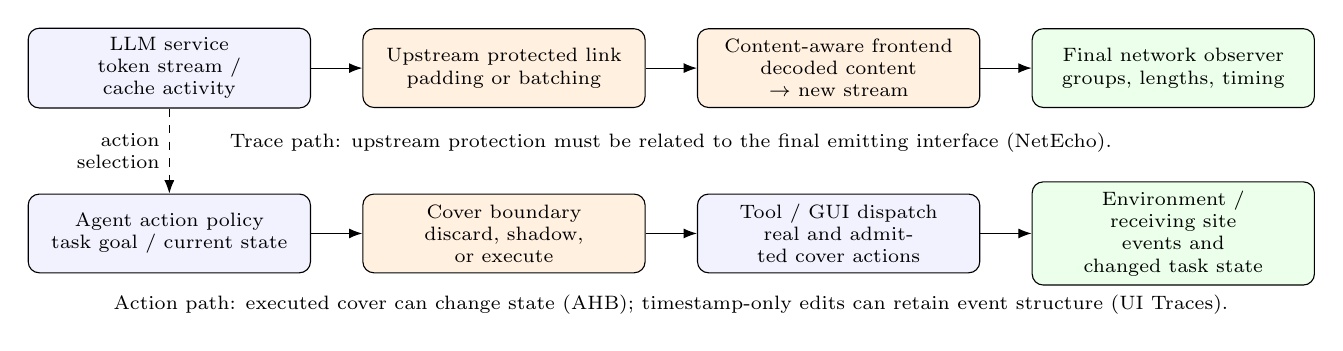
\begin{tikzpicture}[font=\scriptsize,>=Latex,
box/.style={draw,rounded corners,align=center,text width=3.35cm,minimum height=10mm,fill=blue!5},
boundary/.style={box,fill=orange!12},
observer/.style={box,fill=green!8}]
\node[box] (llm) at (0,0) {LLM service\\token stream / cache activity};
\node[boundary] (api) at (4.25,0) {Upstream protected link\\padding or batching};
\node[boundary] (front) at (8.5,0) {Content-aware frontend\\decoded content $\rightarrow$ new stream};
\node[observer] (net) at (12.75,0) {Final network observer\\groups, lengths, timing};
\draw[->] (llm)--(api);
\draw[->] (api)--(front);
\draw[->] (front)--(net);
\node[box] (policy) at (0,-2.1) {Agent action policy\\task goal / current state};
\node[boundary] (cover) at (4.25,-2.1) {Cover boundary\\discard, shadow, or execute};
\node[box] (dispatch) at (8.5,-2.1) {Tool / GUI dispatch\\real and admitted cover actions};
\node[observer] (state) at (12.75,-2.1) {Environment / receiving site\\events and changed task state};
\draw[->] (policy)--(cover);
\draw[->] (cover)--(dispatch);
\draw[->] (dispatch)--(state);
\draw[->,dashed] (llm.south)--node[left,align=right]{action\\selection}(policy.north);
\node[font=\scriptsize,align=center] at (6.37,-.95)
{Trace path: upstream protection must be related to the final emitting interface (NetEcho).};
\node[font=\scriptsize,align=center] at (6.37,-3.0)
{Action path: executed cover can change state (AHB); timestamp-only edits can retain event structure (UI Traces).};
\end{tikzpicture}

\caption{Observation and execution boundaries. The four demonstrations test emitter placement, stateful execution/link composition, real-agent operation signatures, and timing with matched transport controls.}
\label{fig:system-model}
\end{figure*}

\section{Scope and Systematization Method}\label{sec:methodology}\label{sec:background}
\subsection{Research questions, eligibility and threat polarity}
We organize the systematization around four questions. \textbf{RQ1 (landscape):} which hidden targets, threat polarities and auxiliary observables appear across LLM and agent systems, and where is each signal generated versus observed? \textbf{RQ2 (comparability):} when do two reported defense results measure the same target, receiver, intervention and cost object? \textbf{RQ3 (joint evidence):} which results bind protection, utility and cost at one evaluated operating point? \textbf{RQ4 (transfer):} which evidence distinguishes attack generalization, defended-condition evaluation and defense transfer across tasks, models, topologies and hardware? RQ1 supplies the field context; RQ2--RQ4 correspond to the three contributions.

Core inclusion requires five conjunctive criteria: (C1) LLM or agent execution, (C2) a hidden target property, (C3) an execution-dependent auxiliary observable rather than ordinary output semantics alone, (C4) specified observer permissions, and (C5) an empirical inference evaluation. Mixed-feature papers qualify only if they isolate an auxiliary-only C3 component; thus coding fingerprints, WildAuth, ZeroPrint, endpoint-content fingerprints and StepFinder remain adjacent boundary comparators \cite{ghaleb2026codingfingerprint,wang2026dialogue,shao2026zeroprint,leshin2026endpoint,zhu2026stepfinder}. Table~\ref{tab:boundary-rules} states the observable eligibility rules. For C3, the extraction must name an execution mechanism and an evaluated observable separate from ordinary linguistic meaning. A filter qualifies when its accept/reject behavior or differential response is the measured oracle for a hidden property; merely analyzing a reply's wording or style does not. If a mixed paper does not isolate that mechanism, its membership stays adjacent. This operational distinction concerns the measured signal, not whether the output is text.
\begin{table}[t]\centering\footnotesize
\caption{Observable-based eligibility. A hidden target alone does not make a semantic attack a side channel.}\label{tab:boundary-rules}
\begin{tabularx}{\columnwidth}{@{}p{.39\columnwidth}Y@{}}\toprule
Observed input & Decision and required distinction\\\midrule
Length, timing, cache response & Core when measured execution dependence supports hidden-target inference.\\
Own-site actions & Core attribution with site permission; no automatic access to other sites or private tool logs.\\
Reply states the secret & Direct disclosure; adjacent, not auxiliary-channel evidence.\\
Reply style/content identifies a user & Adjacent unless a separately evaluated auxiliary mechanism is established. WildAuth stays a mixed-view comparator.\\
Output-filter membership oracle & Can be core: the filter's execution, not ordinary semantic output inference, mediates the signal.\\
Privileged loop/fault logs & Separate diagnostic component when C1--C5 hold; does not increase confidentiality evidence.\\\bottomrule
\end{tabularx}\end{table}


We use four narrative groupings of objectives and observer roles, not mutually exclusive classes. An unauthorized identity inference can be both attribution and a confidentiality concern. Each record separately specifies the inference target, observer, authorization relation and protected interest:
\textbf{Type I} concerns confidentiality/privacy; \textbf{Type II} concerns model, harness or identity attribution; \textbf{Type III} concerns evasion of a platform's human--agent detector; \textbf{Type IV} concerns authorized operator diagnostics. Types can overlap. WRA protects research intent (I); UI Traces attributes agents (II); AHB evades a defensive detector (III); ClawGuard diagnoses loops (IV) \cite{jeong2026wra,uitraces2026,zhu2026turing,gan2026clawguard}. These roles are mapped per core family, alongside generating and receiving layers, in Table~\ref{tab:core-family-map}.

\subsection{Corpus construction and reconciliation}
Forty seeds, venue-targeted proceedings screening and one-hop citation snowballing produced an initial map of \SnapshotN{} families (\SnapshotCore{} core, \SnapshotAdjacent{} adjacent). A supplementary database and bulk keyword search returned 615 occurrences and 565 unique records; auditing its 204 exclusions rerouted four records, and the search added 15 core and seven adjacent families. The final collection has \FinalCore{} core and \FinalAdjacent{} adjacent families. The completed search frames, closed on October~21, 2026, combine Semantic Scholar and native arXiv queries with venue-targeted screening of S\&P, USENIX Security, NDSS, CCS and PMLR. C1--C5 screening and version deduplication operate on records before family reconciliation; the supplement retains queries, dispositions and excluded incomplete search frames. Architecture and hardware venues were not comprehensively screened; the finite frame is not an exhaustive census.

\subsection{Source-bound result records}
Each record links its target, observation boundary and operating point to a source version and section/table/figure locator. The authors report reviewing the classification of all 82 families using titles, abstracts and experimental sections, and checking all 39 result records and 180 family-audit cells against source locators. The subsequent 351-cell record audit and 133 within-question pair decisions retain author-assigned reasons; executable checks establish their accounting consistency. Candidate fields produced with AI assistance were subject to this author review.

Appendices~\ref{app:records} and \ref{app:reconstruction} contain the record index, comparison summary and query memberships in this PDF. The ledger also separates cited publication status, inspected version, measurement mode and remaining binding uncertainty. Published status increases traceability of venue review but does not establish the correctness of a result; a preprint's observations remain provisional at their inspected scope.

\soktakeaway{SoK Takeaway 1 (Map evidence to the receiving deployment)}{A family-level label does not identify which signal, observer permission or protected objective a result supports. The complete core map separates signal origin from receiving access; the result ledger then binds each comparison to a source version and operating point.}

\section{Result Records, Comparability Rules and Validity}\label{sec:scope}
The atomic unit of our repository is one \emph{evaluated result record}, rather than a whole paper or a single headline score. A result record binds a source version and locator to seven structured fields: Source, Target (and threat polarity Types~I--IV), Receiver projection, Intervention boundary, Attacker training/calibration ($D_0$: clean-condition fit; $D_2$: protected-condition fit), Workload/holdout, and Outcomes (inference metric, task/component utility, and cost object; Table~\ref{tab:result-record}). A study family contributes multiple records whenever it evaluates distinct execution modes (e.g., stored capture vs.\ live loopback in Dangol \cite{dangol2026workflow}), distinct mechanisms (e.g., $K$-prefix KV simulation vs.\ GPTCache semantic de-identification in Early Bird \cite{earlybird2025}), or separately scoped performance benchmarks (e.g., SafeKV \cite{chu2025safekv} and OTRO \cite{lee2026otro}).
\begin{table}[t]\centering\footnotesize
\caption{A single result record. Only fields relevant to the requested comparison must align; unavailable required fields remain unresolved.}\label{tab:result-record}
\begin{tabularx}{\columnwidth}{@{}p{.22\columnwidth}Y@{}}\toprule
Record field & Required meaning\\\midrule
Source & Family/result ID, version, source locator, reading scope and hash.\\
Target & Hidden property, inference goal and protection relation: confidentiality, attribution, human/agent distinction or authorized diagnosis.\\
Receiver & Actual permission and released representation, including session/document linkage and any auxiliary inputs.\\
Intervention & Where protection ends; whether edits affect stored traces, transmission or executed actions.\\
Attacker & Fit/calibration condition, test population, training access and adaptation budget.\\
Workload & Task, system, topology/hardware and grouping/holdout.\\
Outcomes & Inference metric / denominator; objective or proxy utility; applicable cost object; uncertainty and field states.\\\bottomrule
\end{tabularx}\end{table}


\paragraph{Indexing schema and comparison contracts}
The mnemonic \scope{} (Secret/target, Channel, Observer, Pipeline, Exploitation goal) names the target-and-channel columns of our index, paired with evaluation provenance. Generating layers span hardware (P1), serving (P2), transport (P3), application/API (P4), orchestration (P5), tools/MCP (P6), environment (P7) and multi-agent communication (P8). We apply three comparison contracts (Table~\ref{tab:comparison-contracts}): a comparison is \emph{compatible} when required fields align; \emph{incompatible} when a positive mechanism or boundary conflict is established (such as substituting token-payload ratios for wire bytes or offline timestamp edits for live action delays); and \emph{unresolved} when a required binding is unreported (U), unavailable (A) or unverified (?). Table~\ref{tab:result-lineage} illustrates a complete record-to-judgment lineage.
\begin{table}[t]\centering\footnotesize
\caption{Comparison rules. A known mismatch and a missing binding have different consequences.}\label{tab:comparison-contracts}
\begin{tabularx}{\columnwidth}{@{}p{.28\columnwidth}Y@{}}\toprule
Requirement & Condition and resulting license\\\midrule
Descriptive comparison & Align target, receiver permission, metric meaning and cost object. Different systems may be described together; token payload and wire bytes cannot be ranked as the same cost.\\
Paired effect & Compare the same defended test units and outcome. A known test-unit mismatch makes that subtraction incompatible; an unverified fit binding leaves the effect unresolved.\\
Deployment transfer & Establish a bridge for the changed receiver, intervention, workload, topology or hardware. A demonstrated violation blocks the proposed transfer; an untested bridge leaves it unresolved. Permit only the range and endpoints actually covered.\\\bottomrule
\end{tabularx}\end{table}

\begin{table}[t]\centering\footnotesize
\caption{Filled record and its licensed judgment. Values are source-reported; no cross-mode effect is computed.}\label{tab:result-lineage}
\begin{tabularx}{\columnwidth}{@{}p{.24\columnwidth}Y@{}}\toprule
Join key / field & Entry\\\midrule
Family / result & Dangol workflow / \texttt{DANGOL-livebinding}.\\
Version / locator & arXiv:2606.07150v3, \S9.7, live-protocol paragraph after Table~5 \cite{dangol2026workflow}.\\
Target / view & Workflow classification from live Oblivious HTTP (OHTTP)/Agent-to-Agent (A2A) traffic; not GUI-state observation.\\
Intervention & Live fixed-rate cover with fresh per-session identifiers, distinct from transformed stored captures.\\
Workload / testbed & Workflow classes with client, relay, gateway and agent co-located on one loopback host.\\
Outcome / cost & Accuracy 0.30; about $13\times$ bytes and $11\times$ latency in that condition.\\
Unresolved fields & Objective terminal task utility \NRR{}; precise paired live-refit comparison \NRV{}.\\
Licensed judgment & These costs describe this live protocol condition. They neither price dummy GUI actions nor prove task preservation. A matched objective endpoint is needed for the latter.\\\bottomrule
\end{tabularx}\end{table}



\paragraph{Executable comparison rules}
The record schema and comparison contracts precede the audit results. Table~\ref{tab:audit-rules} gives all nine operational rules and a shared evidence-status alphabet; Table~\ref{tab:family-audit} applies them to every mitigation family. Twenty-four constructed cases and seven mechanism checks exercise rule application in the artifact, while the source-linked cases in \S\ref{sec:discussion} explain the substantive comparison judgments.

\section{Corpus Map Across 82 Study Families}\label{sec:corpus-map}
\subsection{Generating layers, receiving projections and threat polarities}
Table~\ref{tab:core-family-map} maps all \FinalCore{} core families by signal-generating layers, receiving projections and threat polarity. Multi-layer families retain every reported layer in their generating and observing sets.
\begin{table*}[!t]\centering\footnotesize
\caption{Complete map of the 58 core study families. Each family appears once; layer and type labels may be multiple and do not imply one-to-one causal paths. The blocks group source layers, not evidential quality.}\label{tab:core-family-map}
\setlength{\tabcolsep}{2pt}
\begin{minipage}[t]{0.49\textwidth}\vspace{0pt}\centering
\begin{tabularx}{\linewidth}{@{}Ycc@{}}\toprule
Core family & $G\,\to\,O$ & Type\\\midrule
\multicolumn{3}{@{}l}{\textbf{hardware generation, P1 (8)}}\\\midrule
Edge EM leakage~\cite{alhalawani2026physicaledge} & $1\,\to\,1$ & \texttt{I}\\
Energon~\cite{chaudhuri2025energon} & $1\,\to\,1$ & \texttt{II}\\
MoEcho~\cite{ding2025moecho} & $1\,\to\,1$ & \texttt{I}\\
I Know What You Said~\cite{gao2025iknow} & $1\,\to\,1$ & \texttt{I}\\
Behind Bars~\cite{gu2026behindbars} & $1\,\to\,1$ & \texttt{I}\\
PAGE404~\cite{nazaraliyev2026page404} & $1\,\to\,1$ & \texttt{I}\\
Spill the Beans~\cite{spillbeans2025} & $1\,\to\,1$ & \texttt{I}\\
ArchSnoop~\cite{weng2026archsnoop} & $1\,\to\,1$ & \texttt{II}\\
\midrule
\multicolumn{3}{@{}l}{\textbf{hardware and service, P1/P2 (8)}}\\\midrule
SparLeak~\cite{chen2026sparleak} & $1,2\,\to\,1$ & \texttt{I}\\
Shape and Substance~\cite{hadad2026shape} & $1,2\,\to\,1$ & \texttt{I}\\
TDXRay~\cite{hornetz2026tdxray} & $1,2\,\to\,1$ & \texttt{I}\\
SparSEEty~\cite{jo2026sparseety} & $1,2\,\to\,1$ & \texttt{I}\\
OTRO~\cite{lee2026otro} & $1,2\,\to\,1$ & \texttt{I}\\
Detokenization Leaks~\cite{weiss2026detokenization} & $1,2\,\to\,1$ & \texttt{I}\\
LLM-WFIN~\cite{jiao2025llmwfin} & $1,2\,\to\,1,3$ & \texttt{I}\\
LLM-serving RCA~\cite{scheinert2026rca} & $1,2\,\to\,2$ & \texttt{IV}\\
\midrule
\multicolumn{3}{@{}l}{\textbf{service generation, P2 (first 13 of 22)}}\\\midrule
SplitDecoy~\cite{politis2026splitdecoy} & $2\,\to\,2$ & \texttt{I}\\
KVGov~\cite{addagada2026kvgov} & $2\,\to\,2,4$ & \texttt{I}\\
LLMs Have Rhythm~\cite{alhazbi2025rhythm} & $2\,\to\,3$ & \texttt{II}\\
Remote timing~\cite{carlini2024remote} & $2\,\to\,3$ & \texttt{I}\\
NetEcho~\cite{netecho2025} & $2\,\to\,3$ & \texttt{I}\\
Prompt Echo~\cite{prompt_echo2026} & $2\,\to\,3$ & \texttt{I}\\
Speculative decoding~\cite{wei2024speculation} & $2\,\to\,3$ & \texttt{I}\\
Remote keylogging~\cite{weiss2024prompt} & $2\,\to\,3$ & \texttt{I}\\
Whisper Leak~\cite{whisperleak2025} & $2\,\to\,3$ & \texttt{I}\\
Cache contention~\cite{abubakar2026contention} & $2\,\to\,4$ & \texttt{I}\\
Routing metadata~\cite{chen2026routingmetadata} & $2\,\to\,4$ & \texttt{I}\\
SafeKV~\cite{chu2025safekv} & $2\,\to\,4$ & \texttt{I}\\
ML privacy channels~\cite{debenedetti2024privacy} & $2\,\to\,4$ & \texttt{I}\\
\bottomrule\end{tabularx}\end{minipage}\hfill
\begin{minipage}[t]{0.49\textwidth}\vspace{0pt}\centering
\begin{tabularx}{\linewidth}{@{}Ycc@{}}\toprule
Core family & $G\,\to\,O$ & Type\\\midrule
\multicolumn{3}{@{}l}{\textbf{service generation, P2 (remaining 9 of 22)}}\\\midrule
Early Bird~\cite{earlybird2025} & $2\,\to\,4$ & \texttt{I}\\
Prompt-cache audit~\cite{gu2025promptcaching} & $2\,\to\,4$ & \texttt{I}\\
InputSnatch~\cite{inputsnatch2024} & $2\,\to\,4$ & \texttt{I}\\
Leaky Language Models~\cite{majidi2026leakylms} & $2\,\to\,4$ & \texttt{I}\\
PromptPeek~\cite{promptpeek2025} & $2\,\to\,4$ & \texttt{I}\\
SpliceLeak~\cite{spliceleak2026} & $2\,\to\,4$ & \texttt{I}\\
Time Will Tell~\cite{timewilltell2024} & $2\,\to\,4$ & \texttt{I}\\
CachePrune~\cite{wu2026cacheprune} & $2\,\to\,4$ & \texttt{I}\\
MoE prompt stealing~\cite{yona2024stealing} & $2\,\to\,4$ & \texttt{I}\\
\midrule
\multicolumn{3}{@{}l}{\textbf{cross-layer sources (5)}}\\\midrule
ClawGuard~\cite{gan2026clawguard} & $1,5\,\to\,1$ & \texttt{IV}\\
MIRAGE~\cite{revankar2026mirage} & $2,5\,\to\,2$ & \texttt{IV}\\
Cloud traffic benchmark~\cite{pouryousef2026traffic} & $2,5,8\,\to\,3$ & \texttt{I,II}\\
Web-agent unmasking~\cite{fayolle2026webagents} & $3,7\,\to\,3,7$ & \texttt{II,III}\\
LumiMAS~\cite{solomon2026lumimas} & $4,5\,\to\,4,6$ & \texttt{IV}\\
\midrule
\multicolumn{3}{@{}l}{\textbf{orchestration/workflow sources (15)}}\\\midrule
AgentPrint~\cite{agentprint2025} & $5\,\to\,3$ & \texttt{I,II}\\
Cycle detection~\cite{george2025cycles} & $5\,\to\,4,6$ & \texttt{IV}\\
SIGLEAK~\cite{geng2026sigleak} & $5,6\,\to\,4,6$ & \texttt{I}\\
ProcGrep~\cite{oderinwale2026procgrep} & $5,6\,\to\,4,6$ & \texttt{II}\\
AgentProv~\cite{wang2026agentprov} & $5,6\,\to\,6$ & \texttt{II}\\
Lidar~\cite{wang2026lidar} & $5,6\,\to\,6$ & \texttt{II}\\
Dangol workflow~\cite{dangol2026workflow} & $5,6,8\,\to\,3,6,8$ & \texttt{I}\\
Campaign attribution~\cite{park2026crosscampaign} & $5,6,8\,\to\,6,8$ & \texttt{II}\\
WRA~\cite{jeong2026wra} & $5,7\,\to\,3$ & \texttt{I}\\
PersonaFingerprint~\cite{song2026personafingerprint} & $5,7\,\to\,3$ & \texttt{I}\\
Whose Agent?~\cite{kang2026whoseagent} & $5,7\,\to\,7$ & \texttt{II}\\
AgentTell~\cite{shahriar2026agenttell} & $5,7\,\to\,7$ & \texttt{I}\\
UI Traces~\cite{uitraces2026} & $5,7\,\to\,7$ & \texttt{II}\\
FP-Agent~\cite{wang2026fpagent} & $5,7\,\to\,7$ & \texttt{II}\\
AHB~\cite{zhu2026turing} & $5,7\,\to\,7$ & \texttt{III}\\
\bottomrule\end{tabularx}\end{minipage}
\par\smallskip\raggedright $G$ denotes signal-generation layers and $O$ the receiving observation layers. Layer indices: 1 hardware; 2 serving/runtime; 3 transport; 4 application/API; 5 orchestration; 6 tools; 7 browser/environment; 8 multi-agent communication. Types: I confidentiality/privacy; II attribution; III human--agent distinction/evasion; IV authorized diagnostics. These are objectives and observer roles, not mutually exclusive security guarantees. Privileged operator receivers and physical receivers are marked by the layer they inspect. Source versions, locators and normalization of prose-only layer descriptions are in the artifact.
\end{table*}


\paragraph{Cross-layer synthesis}
A remote network observer, a same-site script and a privileged diagnostic hook expose different views even when they share an attribution target. WRA's read-only privacy decoys, AHB's stateful evasion and SplitDecoy's exposed return path illustrate why receiving permissions and protected objectives must accompany the generating layer \cite{jeong2026wra,zhu2026turing,politis2026splitdecoy}.

Layer incidence highlights where the systematization's comparison problem arises. In the 58-family map, signal-generation labels cluster at P2 serving/runtime (32 families) and P5 orchestration (19); receiving views cluster at P4 application/API (18), P1 hardware (16), and P3 transport (14). Generation at P3/P4 is rare (one family each), despite frequent observation at those layers. This source/receiver asymmetry makes the transfer question concrete: protection at a frequent source layer cannot be presumed to cover a different receiving projection. The map records layer sets, so it does not assign a causal edge to each source/receiver pair.

Purpose labels further show why a single “agent side channel” category is insufficient: Type I appears 41 times, Type II 13, Type III 2, and Type IV 5. The 32 map-only families extend coverage beyond mitigation comparisons: 15 list serving origins, 11 hardware and 11 orchestration; 19 concern confidentiality, nine attribution, one evasion and all five authorized-diagnostic families. Mapping these families locates privacy targets, operator capabilities and candidate validation environments even when no scoped mitigation record enters the ledger. Counts are overlapping family-label incidences; the audit then applies its reuse rules to the 39 scoped result records.

\subsection{Relationship to prior systematizations}
Prior surveys map compound-system threats, TEE boundaries and privacy contracts \cite{banerjee2024compound,forough2026secrets,kotevska2026privacyfoundations}. WF already supplies feature leakage analysis, cost trade-offs and environment-shift tests \cite{cai2014systematic,juarez2014critical,juarez2016wtfpad,wang2017walkietalkie}. Mathews et al. re-evaluate nine defenses with stronger attacks and an on-network DynaFlow implementation \cite{mathews2023critical}. Adaptive attacks and online-cost evaluation are established foundations.

\paragraph{What this synthesis adds}
Our unit is a \emph{scoped result}, so execution mode, protected state and cost remain attached when one paper reports several mechanisms. The 39-record census exposes these within-paper substitutions; the 82-family holdout matrix separates evidence for each transfer axis. This connects evidence that earlier taxonomies organize by attack or mechanism: one family can contain several execution modes, a receiving projection can cross system layers, and utility/cost can belong to a different operating point from inference. The synthesis preserves these distinctions when translating a reported result into a deployment decision.

\section{Comparability Audit Across All 58 Core Families}\label{sec:defenses}
\subsection{Unified 58-core disposition and 39-record ledger}
The corpus partitions as $82=58$ core $+24$ adjacent families. Within the core, $58=20$ mitigation $+6$ contextual $+32$ map-only families. The ledger holds 39 records: 33 from the 20 mitigation families and one from each contextual family---SIGLEAK, AgentTell, FP-Agent, Behind Bars, LLMs Have Rhythm and ML privacy channels \cite{geng2026sigleak,shahriar2026agenttell,wang2026fpagent,gu2026behindbars,alhazbi2025rhythm,debenedetti2024privacy}---which supply fixed-guardrail, access-control, interference, VPN or filter-origin contrasts rather than an audited mitigation claim. The 32 map-only families comprise 22 without a scoped mitigation evaluation, five diagnostics, four unbound quantitative assertions and SplitDecoy's boundary case. Table~\ref{tab:defense-types} groups mechanisms; its eight rows are mechanism groups, not sampled studies.
\begin{table*}[t]\centering\footnotesize
\caption{Seven privacy and attribution intervention categories organized by receiving view and supported deployment judgment. Type I protects confidentiality; Type II addresses provenance or identity attribution.}\label{tab:defense-types}
\begin{tabularx}{\textwidth}{@{}p{.17\textwidth}p{.29\textwidth}Y@{}}\toprule
Intervention \& polarity & Evaluated view, target and source & Established result and applicable boundary\\\midrule
Padding / batching (Type~I: confidentiality) & Network packet lengths and groups; topic inference. NetEcho and Whisper Leak \cite{netecho2025,whisperleak2025}. & Collected padding traces retain inference signal; packet-group batching is evaluated by replay. A protected upstream length view does not cover downstream re-emission or residual grouping. Live incremental cost remains \NRR{}.\\
Constant-rate / transport cover (Type~I: confidentiality) & Network workflow fingerprint; Dangol's OHTTP testbed \cite{dangol2026workflow}. & The co-located loopback setting yields 0.30 recovery at about $13\times$ bytes and $11\times$ latency. Transformed-capture results are separate; neither result supplies objective agent-task utility.\\
Concurrent query decoys (Type~I: confidentiality) & Destination/domain observer; private prompt and trait inference. WRA \cite{jeong2026wra}. & Real/decoy research prompts execute in parallel as read-only queries whose decoy answers are discarded locally; interleaved-domain evaluation reduces one-decoy $E_{\rm func}$ from 0.770 to 0.610. Terminal decoy utility/cost are \NRR{}.\\
Cache isolation / keying (Type~I: confidentiality) & Co-tenant prefix timing; SafeKV, KVGov and CachePrune \cite{chu2025safekv,addagada2026kvgov,wu2026cacheprune}. & SafeKV reports post-trigger AUC near 0.5 and separate TTFT/throughput comparisons. KVGov's HMAC median $1.3\,\mu$s prices key computation, excluding lost reuse. CachePrune jointly binds marked-token protection, QA/summarization utility and serving performance.\\
Cache timing equalization (Type~I: confidentiality) & Co-tenant cache-fusion timing; SpliceDefense \cite{spliceleak2026}. & Constant-Time Boundary Fusion (CTBF) suppresses the tested signal over 15 tasks/75 steps. Quantized Chunk Padding (QCP) adds mean 7.5 tokens and $<5$ms/$<1\%$ prefill time; this does not price combined deployment.\\
Timestamp perturbation (Type~II: attribution) & Recorded website action metadata; model/agent attribution. UI Traces \cite{uitraces2026}. & Fitting on delayed traces ($D_2$) recovers substantial attribution performance under offline timestamp edits that retain action types/order. Live execution delay and task outcomes are not measured by the trace transformation.\\
Oblivious / unshared memory (Type~I: confidentiality) & Host or local resource observations; TDXRay, Gao et al.\ and OTRO \cite{hornetz2026tdxray,gao2025iknow,lee2026otro}. & TDXRay measures oblivious-map lookup cost; Gao measures loading/memory cost after disabling zero-copy. OTRO reduces conditional access-count information (3.94 to 0.04 bits) with separate unpadded TTFT (4.59\%) and epoch-padding ($2.8$ms) bounds.\\\bottomrule
\end{tabularx}
\par\smallskip\raggedright\footnotesize
Authorized operator diagnostics (Type~IV: ClawGuard, cycle detection, LumiMAS, LLM-serving RCA and MIRAGE) are baseline telemetry rather than privacy attacks or evasion defenses, and are cataloged separately.
\end{table*}

\paragraph{Whole-ledger synthesis}
Each record has one primary measurement mode: 20 executed collections/prototypes, six trace transformations, five simulations/derived estimates, six component/calibration measurements and two unresolved placements (Table~\ref{tab:r9-record-index}). Eleven of the 20 mitigation families contribute more than one record, and nine of them span more than one mode; this is why a mechanism name cannot carry utility or cost between records. Executed collection establishes its stated execution scope, not automatically full-workflow utility.

\subsection{Within-family and within-cohort record comparisons}
The pairwise audit covers the 33 records in the ledger before the final search (27 mitigation, six contextual); the six records that search added contribute two further same-family pairs (\texttt{CACHEPRUNE-selective}/\texttt{-context} and \texttt{OTRO-unpadded}/\texttt{-epochpad}). Of the $\binom{33}{2}=528$ pairs, 426 cross unrelated mechanism cohorts and are out of scope by construction. The remaining 102 related pairs (66 traffic-envelope, 28 cache-service, three behavioral-humanization, three generator-fingerprint, one local-memory, one fixed-instruction) include the 13 same-family pairs. They show why paper-level comparison fails:
\begin{itemize}
\item \textbf{Same paper, different object.} Six of 13 same-family pairs (7 of 15 with the two later pairs) measure different primitives, targets or cost objects, e.g., Early Bird's $K$-prefix oracle simulation versus its GPTCache semantic prototype, or SpliceDefense's CTBF signal suppression versus QCP-only prefill cost.
\item \textbf{Same object, different population.} Of the seven aligned-outcome same-family pairs, four evaluate different collection or execution populations (e.g., Dangol's stored-capture ablation at 0.17 accuracy versus live loopback OHTTP at 0.30) and three lack a verified matched-test binding; none licenses subtraction as a paired deployment effect.
\item \textbf{Across papers.} Of the 102 related pairs, 16 (15.7\%) support a source-qualified descriptive comparison, 80 (78.4\%) have an established receiver, target or cost-object mismatch, and 6 (5.9\%) remain unresolved.
\end{itemize}

\subsection{Nine-item reuse audit across 20 mitigation families}
Table~\ref{tab:audit-rules} defines each item before its application to the 180 cells in Table~\ref{tab:family-audit}. Applicability follows the result's reuse claim: a fixed analytical attack makes adaptation inapplicable, while a component benchmark can support component utility. \NRR{} and \NRV{} retain distinct source states: the 11 unverified cells are five R4 and six R5 bindings, which are distinguished from an attack failure.
\begin{table}[t]\centering\footnotesize
\caption{Operational rules for the nine reuse bindings. Apply each item to a specified result record and deployment claim.}\label{tab:audit-rules}
\begin{tabularx}{\columnwidth}{@{}p{.30\columnwidth}Y@{}}\toprule
Item & Evidence required for a Bound (\textbf{B}) judgment\\\midrule
R1 Target & Hidden property, inference goal and authorized/protected interest are explicit.\\
R2 Receiver & Observer permission, released representation and auxiliary inputs identify the evaluated view.\\
R3 Intervention & Placement and execution mode bind the transform to stored data, wire emission or executed actions.\\
R4 Protected fit & Attacker fitting/calibration uses the protected condition; training and protected testing are identified.\\
R5 Matched adaptation & Clean- and protected-condition fits are evaluated on the same defended test population.\\
R6 Workload & Tasks, system/generator configuration and holdout specify the supported transfer axis.\\
R7 Inference & Metric, denominator and evaluation condition bind the attack outcome to the scoped mechanism.\\
R8 Utility & Task/component performance is measured at the same protected operating point, with its state boundary explicit.\\
R9 Cost & Resource units, baseline and measurement object price that operating point.\\\bottomrule
\end{tabularx}
\par\smallskip\raggedright\footnotesize \textbf{B}: bound; \textbf{P}: partial binding; \NRR{}: unreported in inspected scope; \NRA{}: source unavailable; \NRV{}: binding unverified; --: inapplicable. First determine applicability, then assign evidence status. Family \textbf{B} means at least one scoped record satisfies the item, not that every result does.
\end{table}

\begin{table}[t]\centering\footnotesize
\caption{Record-derived evidence availability for all 20 evaluated-mitigation families. R1--R9 are scoped reuse items, not overall paper scores.}\label{tab:family-audit}
\setlength{\tabcolsep}{2.2pt}
\begin{tabularx}{\columnwidth}{@{}Y*{9}{c}@{}}\toprule
Family & R1 & R2 & R3 & R4 & R5 & R6 & R7 & R8 & R9\\\midrule
UI Traces~\cite{uitraces2026} & \textbf{B} & \textbf{P} & \textbf{B} & \textbf{B} & \textbf{B} & \textbf{B} & \textbf{B} & U & --\\
WRA~\cite{jeong2026wra} & \textbf{B} & \textbf{P} & \textbf{B} & -- & -- & \textbf{P} & \textbf{B} & \textbf{P} & U\\
NetEcho~\cite{netecho2025} & \textbf{B} & \textbf{B} & \textbf{B} & \textbf{B} & ? & \textbf{B} & \textbf{B} & U & \textbf{P}\\
Early Bird~\cite{earlybird2025} & \textbf{B} & \textbf{B} & \textbf{B} & \textbf{B} & ? & \textbf{B} & \textbf{B} & U & \textbf{B}\\
Whisper Leak~\cite{whisperleak2025} & \textbf{B} & \textbf{B} & \textbf{B} & \textbf{P} & U & \textbf{B} & \textbf{B} & U & \textbf{P}\\
SpliceLeak~\cite{spliceleak2026} & \textbf{B} & \textbf{B} & \textbf{B} & -- & -- & \textbf{B} & \textbf{B} & U & \textbf{B}\\
Time Will Tell~\cite{timewilltell2024} & \textbf{B} & \textbf{B} & \textbf{B} & \textbf{P} & U & \textbf{B} & \textbf{B} & U & \textbf{B}\\
I Know What You Said~\cite{gao2025iknow} & \textbf{B} & \textbf{B} & \textbf{B} & -- & -- & \textbf{P} & -- & -- & \textbf{B}\\
Speculative decoding~\cite{wei2024speculation} & \textbf{B} & \textbf{B} & \textbf{P} & \textbf{P} & U & \textbf{B} & \textbf{B} & -- & \textbf{B}\\
Dangol workflow~\cite{dangol2026workflow} & \textbf{B} & \textbf{B} & \textbf{B} & \textbf{B} & \textbf{B} & \textbf{B} & \textbf{B} & U & \textbf{B}\\
Cloud traffic benchmark~\cite{pouryousef2026traffic} & \textbf{B} & \textbf{P} & \textbf{B} & U & U & \textbf{P} & \textbf{B} & \textbf{P} & U\\
Remote timing~\cite{carlini2024remote} & \textbf{B} & \textbf{B} & \textbf{P} & -- & -- & \textbf{B} & -- & U & \textbf{B}\\
TDXRay~\cite{hornetz2026tdxray} & \textbf{B} & \textbf{B} & \textbf{B} & -- & -- & \textbf{B} & -- & \textbf{B} & \textbf{B}\\
SafeKV~\cite{chu2025safekv} & \textbf{B} & \textbf{B} & \textbf{B} & -- & -- & \textbf{B} & \textbf{B} & U & \textbf{P}\\
AHB~\cite{zhu2026turing} & \textbf{B} & \textbf{B} & \textbf{B} & \textbf{P} & U & \textbf{B} & \textbf{B} & \textbf{B} & U\\
KVGov~\cite{addagada2026kvgov} & \textbf{B} & \textbf{B} & \textbf{B} & -- & -- & \textbf{B} & \textbf{B} & U & \textbf{B}\\
CachePrune~\cite{wu2026cacheprune} & \textbf{B} & \textbf{B} & \textbf{B} & -- & -- & \textbf{B} & \textbf{B} & \textbf{B} & \textbf{B}\\
OTRO~\cite{lee2026otro} & \textbf{B} & \textbf{B} & \textbf{B} & -- & -- & \textbf{B} & \textbf{B} & -- & \textbf{B}\\
SparLeak~\cite{chen2026sparleak} & \textbf{B} & \textbf{B} & \textbf{B} & \textbf{P} & U & \textbf{B} & \textbf{B} & \textbf{B} & U\\
Shape and Substance~\cite{hadad2026shape} & \textbf{B} & \textbf{B} & \textbf{P} & U & U & \textbf{B} & \textbf{P} & U & \textbf{P}\\
\midrule Bound & 20 & 17 & 17 & 4 & 2 & 17 & 16 & 4 & 11\\
Applicable & 20 & 20 & 20 & 11 & 11 & 20 & 17 & 17 & 19\\
\bottomrule\end{tabularx}
\par\smallskip\raggedright \textbf{B}: bound; \textbf{P}: partial; U: unreported in inspected scope; ?: unverified binding; --: inapplicable. Table~\ref{tab:audit-rules} defines R1--R9. Each cell is generated from the scoped records: B if any record is B, otherwise P, ?, U, A, then --. This availability summary retains a witness for every B; separate cells can refer to different configurations. NetEcho and Early Bird retain unresolved record-specific R5 bindings. Dangol's B in R5 is supported by stored capture; its live binding remains unresolved. S36 records the projection and its 13 corrections.
\end{table}


\soktakeaway{SoK Takeaway 2 (Inference is bound; reuse is not)}{Target and inference are bound almost everywhere (R1 20/20, R7 17/20). The bindings needed to carry a result elsewhere are not: protected fit 4/11 applicable families, matched adaptation 2/11 (2/10 for learned adaptive attacks only), utility at the protected operating point 3/17 (2/16 counting task utility only) and cost 11/19. CachePrune alone binds inference, utility and cost at one operating point, and it does not establish adaptation. These are scope sensitivities, not quality ranks.}

\section{Which Evidence Supports Defense Transfer?}\label{sec:evaluation}\label{sec:threats}
\subsection{Separate the evaluated object before counting holdouts}
RQ4 distinguishes three questions: does an \emph{attack} recognize new inputs or systems; is a \emph{defense condition} evaluated; and does a \emph{fixed attacker or defense calibration} carry from a specified source to a target? Table~\ref{tab:r26-transfer-objects} makes the distinction operational. Repeating a defense on several models can establish condition-specific outcomes without establishing a held-out model or transferring a fitted calibration.
\begin{table}[t]\centering\footnotesize
\caption{Three evidence objects for RQ3. The same family may supply several objects in separate experiments.}\label{tab:r26-transfer-objects}
\begin{tabularx}{\columnwidth}{@{}p{.24\columnwidth}YY@{}}\toprule
Object & Required link & Permitted reuse\\\midrule
Attack generalization & Training/profiling source $\to$ held-out inputs or systems; attack outcome. & An attacker or recognition method covers the stated target domain.\\
Defended condition & Named mechanism, local fitting, defended test and outcome. & Retain that operating point; multi-model testing alone is not held-out transfer.\\
Defense transfer & Source-selected policy/calibration held fixed $\to$ target; local-calibration comparator and attacker fit specified. & Transport the evaluated policy only over the tested direction and scope.\\\bottomrule
\end{tabularx}\end{table}


The 82-family matrix in Appendix~\ref{app:holdouts} is a discovery index for these questions. Its six axes are task/input/user, model, harness/topology, hardware, network/load and time. H marks reported separation, V condition variation/recalibration, X a scoped restriction, and ? unresolved extraction. The 13 task/input H entries include only four mitigation families; all three model H entries concern attack/identification generalization in families outside the 20-family mitigation audit. The two topology H entries occur in mitigation families, but their held-out objects are workflow recognizers. These counts therefore cannot be read as 13 task-transfer or three model-transfer validations of defenses. S34 identifies each H entry and its evidence object; S28 preserves the full matrix and source scopes.

\subsection{A changed generator and a tested defense are different bindings}
LLM-Fin, ArchSnoop and LeakyLMs evaluate recognition of unseen model variants or architectures \cite{nazari2024llmfin,weng2026archsnoop,majidi2026leakylms}. This supplies attack-side model generalization. In the traffic benchmark, graph-to-star and star-to-graph classification explicitly move the fitted attacker across topologies; the prompt/temperature countermeasures are separate evaluations \cite[V-B--C]{pouryousef2026traffic}. Dangol's leave-composition-out test likewise examines recognition of a novel workflow shape, separately from its protected-capture frontier \cite[9.8--9.12]{dangol2026workflow}. Neither topology entry licenses a transported defense calibration.

There is nevertheless useful \emph{defense-side variation} evidence. Time Will Tell applies the same fixed-length instruction to two models and reports different residual classification ASRs; this tests a common rule under changed generators \cite[VII-B]{timewilltell2024}. Whisper Leak evaluates mitigation conditions across provider-models, while its prompt holdout describes the classifier protocol \cite[3.2,6]{whisperleak2025}. Preserve those per-condition results; a shared rule, a refitted local attack, a source-trained attack and a source-calibrated defense are four distinct comparisons.

\paragraph{Deployment decision}
For the proposed change, name the source, target, held-out unit, quantities held fixed or refitted, and protected outcome. Carry forward only the corresponding binding. An attack-generalization result justifies including that attacker at the target; a defended-condition result supplies its local outcome; a source-to-target defense-calibration result supports only the stated transfer. This prevents both overclaiming portability and discarding useful local evidence. Unresolved hardware/time entries in the discovery matrix identify source follow-up, not absent experiments.

\section{Synthesis: From Evidence to Reuse Decisions}\label{sec:discussion}
\begin{table*}[t]\centering\footnotesize
\caption{Claim-conditioned reuse decisions derived from the record and holdout audits. Each changed boundary identifies the evidence that must be bound before carrying a result forward.}\label{tab:r19-decisions}
\begin{tabularx}{\textwidth}{@{}p{.17\textwidth}p{.29\textwidth}Y@{}}\toprule
Reuse question & Evidence decision & Retain or measure next\\\midrule
Emitter / representation & An upstream or buffered capture can differ from the final receiving trace and delivery schedule. & Bind inference to the final receiver; retain the emitter's overflow, byte and delivery-delay scope (R2/R3/R9; \S\ref{sec:discussion}).\\
Read cover $\rightarrow$ writes & Discarding a reply does not establish unchanged commits, authorization or workflow outcomes. & Bind the protected state and utility to the executed intervention; include cover calls, quotas and failures (R3/R8/R9).\\
Customer / model calibration & A reported split can separate inputs without changing the generator or calibration population. & State held-out units and calibration provenance; separate local fitting variability from source/domain changes; evaluate the requested transfer axis (R5/R6; \S\ref{sec:evaluation}).\\
Attacker observation & An outcome for one projection or fitted attacker does not supply a result for a richer receiving view. & Evaluate comparable defended tests under the intended observation and adaptation contract; retain receiver-specific inference metrics (R2/R5/R7).\\
Stored trace $\rightarrow$ online path & A trace transformation or simulated span does not measure executed queues, completion or online latency. & Bind the receiver, harness and resource denominator to the online condition; establish the relevant topology/network holdout (R3/R6/R9).\\
Bound cache-reuse package & Early Bird prefix recovery and CachePrune direct recovery permit a scoped candidate comparison; CachePrune binds a shared utility/cost package. & Retain that package for its measured configuration; measure prefix-policy serving cost separately, and re-evaluate any changed workload/hardware.\\
Component $\rightarrow$ workflow utility & Component quality or logical state conformance does not determine a planner's response to scheduling and deadlines. & Report utility at the requested workflow boundary and the same intervention/configuration as protection and cost (R3/R8/R9).\\\bottomrule
\end{tabularx}\end{table*}

The census (\S\ref{sec:defenses}) covers all 39 records and the holdout matrix (\S\ref{sec:evaluation}) all 82 families. We now select three examples by the \emph{comparison decision} they expose, not by effect size: a changed receiving path, cover with different state effects, and an adaptation/cost mismatch within a named mechanism. Their value is the decision they change: retain an aligned result, separate a wrongly joined package, or require a result at a changed execution boundary.

\subsection{Case 1: bind the final target-bearing emitter}
NetEcho's upstream packet-size shaping operates on a different projection from the tool-call sequence. Its plaintext-aware frontend then emits a new size trace (grouped token counts or character lengths), reopening a size channel after upstream protection \cite{netecho2025}. SplitDecoy is a separate return-path record: the cloud sees nonzero gradient row support on every tested frame across nine seeds \cite[Sections 5.1--5.3]{politis2026splitdecoy}. Both change the receiver boundary and therefore require a separately bound inference result.

The data processing inequality requires $S\to Z\to Y$: target-oblivious postprocessing cannot increase $I(S;Z)$ \cite[Theorem~2.8.1]{cover2006elements}. Plaintext-aware re-emission or backward computation breaks that premise. The literature comparison must therefore bind both the final receiving projection and the emitter whose costs are measured.

\subsection{Case 2: resolve the WRA versus AHB cover asymmetry}
WRA's one-decoy $E_{\rm func}$ drops from 0.770 to 0.610, whereas AHB's Trip Planning success falls from 0.75 to 0.15 under \texttt{Online+Fake} humanization \cite{jeong2026wra,zhu2026turing}. Grouping both as ``cover traffic'' conceals different objectives and executions.

WRA discards decoy reads for Type~I confidentiality; AHB executes GUI events for Type~III evasion, potentially navigating or submitting forms. Their utility outcomes are not contradictory, and AHB's missing condition-specific denominators preclude a matched causal effect. A shared workflow setting does not establish shared state effects. Terminal-state reward and dispatch-time authorization also answer different questions: an unconfirmed write can still reach the intended final state. Reuse requires an explicit state/authorization outcome at the intervention being carried forward.

\subsection{Case 3: bind adaptive retraining and cost objects}
A matched adaptation contrast compares clean-trained $D_0$ and defense-trained $D_2$ on identical defended tests. UI Traces and Dangol raise the record-binding question this leaves open: whether a refit, a measured delay and a utility outcome refer to the same executed condition \cite{uitraces2026,dangol2026workflow}. Cost objects show the same pattern. Early Bird's $6$ms/$4\%$ GPTCache cost does not price $K$-prefix isolation; KVGov's $1.3\,\mu$s HMAC microcost omits lost reuse; SpliceDefense's QCP cost does not price CTBF+QCP \cite{earlybird2025,addagada2026kvgov,spliceleak2026}. CachePrune binds protection, QA/summarization utility and throughput, while OTRO separates conditional leakage from TTFT/padding costs \cite{wu2026cacheprune,lee2026otro}. The reuse decision follows the evaluated configuration: retain each source's bound outcome, and request the missing adaptation, execution or cost measurement before extending it.


\subsection{A positive reuse path: from comparison to a candidate configuration}
The Early Bird $K$-prefix record and CachePrune's direct-recovery record form one of the 17 descriptive matches: both address sensitive-token recovery through cache-reuse probes \cite[V-A]{earlybird2025}, \cite[5.1--5.6]{wu2026cacheprune}. This permits an analyst to retain both mechanisms as candidates for that threat, while keeping the oracle and executed-serving measurements separate. The joint audit then changes the next step. CachePrune supplies a default configuration package linking recovery, generation quality and serving cost; the analyst can use that package for a source-scoped feasibility assessment. Early Bird's semantic-cache overhead cannot price its $K$-prefix candidate, so that candidate still needs a serving-cost measurement. Neither a pooled recovery ranking nor a new-hardware guarantee follows from this comparison.

\paragraph{What the three findings add}
Record-level comparison turns a mechanism-level shortlist into correctly scoped alternatives. Configuration-level joint binding distinguishes a reusable package from borrowed utility or cost. Deployment decisions then identify the changed object and the measurement it needs. Compared with established WF practice on adaptive attacks, shifts and online costs \cite{juarez2014critical,mathews2023critical}, the LLM/agent synthesis makes three additional joins explicit: prefix versus semantic-cache primitives, discarded read outputs versus executed state changes, and component generation quality versus planner outcomes. The contribution is the source-backed decision change, not a new information-processing theorem.

\subsection{A deployment query determines the evidence to retain}
Start with the intended receiver, protected outcome and intervention. Record-level comparison identifies whether the cited result measures that object. Configuration-level joint binding identifies which inference, utility and cost outcomes share its configuration. Deployment decisions use the holdout matrix to identify evidence for the proposed change and specify the remaining measurement. Table~\ref{tab:r19-decisions} makes these outputs operational: a new emitter needs a receiver-specific capture, writes need state/authorization checks, source-calibration comparisons need a local fitting-variability control, and an online scheduler needs its own planner utility and latency measurement. The calibration control follows from the comparison design: changing the source can also change the finite training sample used to fit the defense.

Appendix~\ref{app:case-study} applies this procedure in one compact case study. The literature audit and the decision table establish the SoK contribution; the case study provides a worked application with separately scoped measurements.

\section{Testing Defense Transfer Boundaries}\label{sec:controlled-placement}\label{sec:tau-cover-bridge}
Four experiments instantiate the boundaries of \S\ref{sec:discussion} using saved LLM responses and a retail agent workload: the emitter (Exp~1), executed state (Exp~2), calibration population (Exp~3) and attacker observation (Exp~4). Exps~1--2 reproduce known mechanisms to measure their streaming-cost and state/link consequences; Exps~3--4 measure agent-specific operating points. Table~\ref{tab:r7-cohorts} separates populations; Appendix~\ref{app:experiments} indexes all studies.

\paragraph{Shared measurement conventions}
A byte-transparent relay captures post-handshake TLS application records on loopback; TLS~1.3 session tickets are disabled. Standard-prompt results use the arm called \texttt{baseline} in the artifact; \emph{undefended} denotes transport without a program defense. Balanced accuracy (BA) averages the two class recalls. We report the maximum over each specified attack suite and recompute that maximum in each of 2,000 common bootstrap draws, grouping tasks for reference-program tests and customers for real-agent tests. The original protocol's engineering screen requires an upper 95\% BA bound below 0.60 and maximum AUROC below 0.65 for both targets. No defended configuration in Exps~3--4 passes it, so we report paired reductions against named suites rather than absolute protection (\S\ref{sec:validity}).

\paragraph{Attack suites}
Because BA is a suite maximum, every number is indexed by its suite. The \emph{frozen suite} (Exp~3 frozen) contains clean-trained $D_0$, defended-refit $D_2$ and training-derived decoder/count rules over lengths and order. The \emph{11-attack union} (Exp~3 cross-fit and localization) adds learners including a 1D-CNN and a k-FP-style forest-leaf model. The \emph{endpoint suite} (Exp~3 replications and transfer) adds a total-exchange-count rule to six attacks inherited from the frozen protocol (majority, clean- and defended-trained learners, decoded-tool and target-call-count rules). In Exp~4, the \emph{common seven} are learners shared with the offline WF adaptations, and the \emph{full union} (17--22 attacks) adds timing features and learned flush removal.
\begin{table}[t]\centering\footnotesize
\caption{Cohort, observation and cost denominators for Exps~3--4. Standard-prompt pairs: cancel/return BA (\%). Byte ratios price joint shaping against each study's own undefended serialization.}\label{tab:r7-cohorts}
\begin{tabularx}{\columnwidth}{@{}lYrr@{}}\toprule
Study & Observation / attack suite & Undef.\ BA & Joint B$\times$\\\midrule
Exp~3 frozen & Replay lengths/order; frozen suite & 97.2/94.0 & 15.39\\
Exp~3 cross-fit & Analytic lengths/order; 11-attack union & 91.7/85.5 & 19.76\\
Exp~4 & New RPC envelope; lengths/order/time; full union & 91.7/86.4 & 15.11\\\bottomrule
\end{tabularx}
\par\smallskip\raggedright\footnotesize Frozen-split and Exp~4 rows: 276 test episodes, 24 customers, 5/7 positive customers. Exp~3 cross-fit: 690 episodes, 53 customers, 14/18 positive customers. Each prompt has half the episodes. Cross-fit fold calibration yields larger templates ($5.04\times$ calls); frozen-split and Exp~4 rows use $3.83\times$. Repeats measure execution variation within these customer groups.
\end{table}


\subsection{Exp 1: bind protection and cost to the emitter}\label{sec:exp-emitter}
Buffered tests use brief/expanded saved responses for 24 topics (12 training, 12 test). Padding only the upstream link leaves verbosity 100\% separable at a plaintext-aware terminal emitter; padding both reduces BA to 50\%, reproducing NetEcho's mechanism~\cite{netecho2025}. A training-fitted buffered cap achieves 50\% at 2.18$\times$ wire bytes under TLS~1.2 (2.19$\times$ under TLS~1.3).

Streaming the same 48 texts as per-token server-sent events changes the cost contract~\cite{weiss2024prompt,whisperleak2025}. Per-event padding retains token count and 100\% verbosity inference. Eight-token batching cuts bytes to 0.21$\times$ and clean-trained BA to 50\%, yet defended-data refitting restores 100\%. Constant shape reaches 50\% at 2.42$\times$ bytes and 208 versus 105 token intervals; two overflowing test outputs remain identifiable (Table~\ref{tab:transfer-streaming}).
\begin{table}[t]\centering\footnotesize\setlength{\tabcolsep}{1.9pt}
\caption{Exp 1: the same 48 saved responses emitted by a buffered or a token-streaming frontend (TLS~1.3 loopback captures). Bytes are relative to the unpadded emitter of the same kind. TTFB/Done: first and last delivered byte in token intervals (accounting proxy). Accuracies on 24 held-out outputs (12 topics); ID: closed-world top-1 identification among 48 responses (chance 2.1\%).}\label{tab:transfer-streaming}
\begin{tabular}{@{}lrrrrrrr@{}}\toprule
& & & & \multicolumn{2}{c}{Verbosity} & \multicolumn{2}{c}{Prefix}\\\cmidrule(lr){5-6}\cmidrule(l){7-8}
Emitter / framing & Bytes$\times$ & TTFB & Done & $D_0$ & $D_2$ & $D_2$ & ID\\\midrule
Buffered, unpadded & 1.00 & 105 & 105 & 100.0 & 100.0 & 91.7 & 87.5\\
Buffered, training cap & 2.19 & 105 & 105 & 50.0 & 50.0 & 50.0 & 2.1\\
Stream, per token & 1.00 & 1 & 105 & 100.0 & 100.0 & 87.5 & 100.0\\
\quad+ random event pad & 1.29 & 1 & 105 & 100.0 & 100.0 & 87.9 & 62.3\\
\quad+ constant event size & 1.23 & 1 & 105 & 100.0 & 100.0 & 87.5 & 58.3\\
8-token batches, const. & 0.21 & 8 & 105 & 50.0 & 100.0 & 87.5 & 20.8\\
Const.\ events + count cap & 2.42 & 1 & 208 & 50.0 & 50.0 & 50.0 & 6.3\\\bottomrule
\end{tabular}
\par\smallskip\raggedright\footnotesize $D_2$ is the best of total-byte threshold, record-count threshold and a logistic sequence model, each fitted on defended training outputs. Random padding: 10 socket-measured draws plus an independent profiling run. TLS~1.2 gives identical accuracies and byte ratios within 0.03. Verbosity contrasts brief/expanded outputs; Prefix contrasts the first two/three sentences of each expanded output. Tokens use \texttt{o200k\_base}. Training count caps are 208/88 events, with 2/24 and 5/24 test overflows, respectively.
\end{table}

\textbf{Finding.} The same saved content yields different protection and delay under buffering and streaming. A buffered cap's byte ratio cannot price a streaming deployment, whose first-output delay and emission schedule are different outcomes.

\subsection{Exp 2: compose state preservation with link protection}\label{sec:exp-state}
\paragraph{Execution boundary}
Among 115 public retail tasks, 97 have an initially pending order for the task user. Three order-selection seeds yield 291 cover placements before the reference program. Same-item modification changes status and appends a refund in 173 placements despite unchanged item and price; the other 118 calls fail the variant-availability check. Idempotence, $f(f(s,a),a)=f(s,a)$, therefore differs from state preservation, $f(s,a)=s$. Cancelling another user's order changes the shared database. The shadow executor isolates cover effects on a separate state and suppresses its responses; a live-execution control exposes the resulting side effects.

The dispatch observer sees ordered tool names and response lengths. Policies add cancellation, pad its count, interleave donor programs or equalize all tool counts; donors/templates use the known 115-program population. Task-grouped five-fold attacks fit clean/defended gradient boosting and logistic regression on counts, bigrams and lengths, with a count-rule baseline and three seeds (18/32 positive cancellation/return tasks).
\begin{table}[t]\centering\footnotesize\setlength{\tabcolsep}{3pt}
\caption{Exp 2 dispatch results: all 115 reference programs, three seeds, known-population defense calibration; task-folded attackers. Maximum BA (cancel/return); extra calls per real call; database equality with the unprotected run.}\label{tab:r7-e6}
\begin{tabularx}{\columnwidth}{@{}Yrrr@{}}\toprule
Policy & BA (\%) & Calls+ & DB eq.\\\midrule
No cover & 100.0/100.0 & 0.00 & 100\%\\
Cancel, $p=.5$ & 86.1/100.0 & .10 & 100\%\\
Cancel, $p=1$, shadow & 100.0/100.0 & .20 & 100\%\\
Cancel, $p=1$, live & 100.0/100.0 & .20 & 0\%\\
Cancel count $\to2$ & 76.9/100.0 & .35 & 100\%\\
One decoy program & 91.9/85.9 & 1.01 & 100\%\\
Two decoy programs & 83.5/78.1 & 1.98 & 100\%\\
Shape equalization & 50.0/54.5 & 6.71 & 100\%\\\bottomrule
\end{tabularx}\end{table}

One inserted cancellation drives clean-trained BA to chance, while refitting restores 100\%. Count equalization removes that rule's signal, but correlated tools retain 76.9\% BA. Donor programs, inspired by WRA's discarded retrieval cover~\cite{jeong2026wra}, leave 83.5--91.9\%. Shape equalization reaches 50.0/54.5\% at 6.7 extra calls per real call (Table~\ref{tab:r7-e6}). Shadow checks match the original live state in every case; live cancellation changes it in every case.

\paragraph{Final network view}
Four cover policies and three framing choices produce 4,140 TLS~1.2 sessions. The network observer receives direction-tagged record lengths and order. A training-fold profiler maps request sizes to tool types before applying dispatch attacks: request-only identification reaches 89.9/91.4\% (582 calls; majority 29.4\%). Per-call buckets leave return BA at 73.9\%; joint shape cover and constant framing reduce cancellation/return to 54.4/50.0\%, at 26.3$\times$ bytes and 7.7$\times$ calls.

\textbf{Finding.} Call-level cover and per-call framing address complementary observables. Full constant-rate transport can instead hide packet counts from a passive link observer without executing dummy tools~\cite{rfc9347}; Exp~4 measures that alternative. At a dispatch view after decapsulation, cover requires hidden markers and routing to the trusted isolated executor (\S\ref{sec:deployment}). The intervention must match the receiver and the protected state.

\subsection{Exp 3: real-agent signatures and calibrated shaping}\label{sec:real-agent}\label{sec:r5}
\paragraph{Task and collection}
The targets are the reference program's requested operations, \texttt{cancel\_pending\_order} and \texttt{return\_delivered\_order\_items}. This operational target tests whether encrypted metadata reveals which service action a task requests. GPT-6.1 Sol/low plans from public retail policies, schemas and actual sandbox observations; a separate context simulates the user. Two prompts and three repeats on 115 tasks yield 690 runs from 53 customers. The rules prompt adds a customer-details read before order access and a read before each write.

\paragraph{Frozen calibration and behavioral control}
All 414 training runs (69 tasks) precede freezing shared cover templates, donors and framing caps. The 276 test runs cover 46 tasks from 24 disjoint customers. Prefix-only scheduling inserts training-derived cover, flushing unmet counts at episode end. Four program conditions per prompt give 2,760 local TLS replays with lengths/order attacks; every failure and handoff remains included. Real-call pass-through plus isolated cover preserves the logical response/state projection (Appendix~\ref{app:equivalence}); reusing trajectories pairs the network interventions on identical model decisions.

Rules raise read-order adherence from 86.2\% to 97.1\%, while undefended category inference remains above 93\%. Native rewards are 110/138 and 105/138 (paired difference $-3.6$ points, 95\% interval $[-9.5,1.4]$). Thus compliance and metadata privacy separate in the same task population.
\begin{table*}[t]\centering\small
\caption{Exp 3, frozen calibration: operation-category inference on real-agent trajectories. Testing covers 46 tasks from 24 held-out customers, two prompts and three repeats (276 episodes). Network BA is the maximum over the frozen attack suite, with customer-cluster 95\% intervals.}\label{tab:r4-primary}
\begin{tabular}{@{}lrrrrr@{}}\toprule
Condition & Cancel BA [95\% CI] & Return BA [95\% CI] & Original reward (\%) & Bytes$\times$ & Calls$\times$\\\midrule
Undefended & 97.2 [90.0, 100.0] & 94.0 [85.8, 100.0] & 79.7 & 1.00 & 1.00\\
Rules prompt & 97.2 [90.0, 100.0] & 93.5 [85.0, 99.5] & 76.1 & 1.00 & 1.00\\
Padding only & 66.1 [50.0, 83.9] & 55.5 [50.0, 73.0] & -- & 4.02 & 1.00\\
Shape only & 60.8 [55.4, 71.3] & 51.9 [50.5, 57.8] & -- & 4.16 & 3.83\\
Joint program & 50.0 [50.0, 60.6] & 50.0 [50.0, 65.5] & -- & 15.39 & 3.83\\
Rules + joint & 50.0 [50.0, 65.1] & 60.6 [50.0, 73.3] & -- & 15.72 & 3.88\\
\bottomrule\end{tabular}
\par\smallskip\raggedright \textbf{Paired joint-minus-undefended BA differences (percentage points):} standard-prompt cancellation $-47.2$ [$-50.0$, $-33.3$], return $-44.0$ [$-48.9$, $-27.8$]. These post hoc contrasts use the same customer draws and reselect the attack-suite maximum in each condition. Joint = online shadow cover plus constant framing; padding/shape ablations use standard-prompt trajectories. Ratios use undefended transport within each prompt. Shadow isolation preserves the logical planner transcript; the four program conditions replay actual LLM trajectories over local TLS~1.2. Reward is reported only for original model executions; dashes denote no new live defended-planner reward measurement (\S\ref{sec:validity}).
\end{table*}

Joint cover and framing reach 50.0/50.0\% point BA, compared with 97.2/94.0\% undefended, a paired decrease of 47.2/44.0 points (Table~\ref{tab:r4-primary}). Their upper bounds (60.6/65.5\%) fail the screen, and the rules-arm joint return point is 60.6\%, identifying prompt/cohort sensitivity.

\paragraph{Customer-grouped exploratory comparison}
Five-fold cross-fitting refits templates, donors, caps and all attackers on other customers, pooling the full known cohort (14/18 positive customers). The analytic TLS model matches all 2,760 saved sessions and 120 additional captures. Under the 11-attack union, joint constant shaping reduces BA by 31.2/30.0 points (paired 95\% intervals [15.3,41.0]/[14.8,39.2]); buckets reduce it by 34.6/32.8 points, at lower byte cost (Table~\ref{tab:r5}).
\begin{table}[t]\centering\footnotesize\setlength{\tabcolsep}{2pt}
\caption{Exp 3: exploratory cross-fit comparison under the 11-attack union: all 690 episodes and 53 customers. Maximum network BA with customer-bootstrap 95\% intervals. Standard prompt unless marked Rules; byte/call ratios relative to undefended transport.}\label{tab:r5}
\begin{tabular}{@{}lrrr@{}}\toprule
Configuration & Cancel BA (\%) & Return BA (\%) & B$\times$/C$\times$\\\midrule
Undefended & \mbox{91.7 [82.1, 100.0]} & \mbox{85.5 [76.7, 93.4]} & 1.0/1.0\\
Joint constant & \mbox{60.5 [52.9, 72.4]} & \mbox{55.5 [51.8, 64.2]} & 19.8/5.0\\
Joint buckets & \mbox{57.1 [50.0, 71.5]} & \mbox{52.7 [50.0, 61.7]} & 12.4/5.0\\
Rules + buckets & \mbox{56.9 [50.2, 71.2]} & \mbox{52.7 [50.0, 65.0]} & 12.4/5.0\\
\bottomrule\end{tabular}
\par\smallskip\raggedright\footnotesize Joint constant is the frozen study's shadow-count plus constant-framing design, refit within each fold. Joint buckets changes framing to 1024-byte buckets. Every bootstrap draw reselects the complete maximum. Intervals condition on fitted predictions.
\end{table}


\paragraph{Locate the observable operation signature}
An oracle selects write exchanges using true tool types, then exposes only ciphertext lengths/order. Writes comprise 19.6\% of real calls yet retain 91.7/84.9\% BA; removing them leaves 62.8/59.9\% (Table~\ref{tab:r7-e12}). The target names an operation, so the result locates its metadata signature. It directs protection toward specific exchanges, while residual read inference shows why hiding one named call is insufficient.
\begin{table}[t]\centering\footnotesize\setlength{\tabcolsep}{2pt}
\caption{Exp 3 oracle localization under the 11-attack union. Standard prompt: 345 cross-fitted episodes, 53 customers. Maximum network BA (\%) with customer-bootstrap intervals.}\label{tab:r7-e12}
\begin{tabular}{@{}lrrr@{}}\toprule
Target & Full trace & Writes removed & Writes only\\\midrule
Cancel & \mbox{91.7 [82.1, 100.0]} & \mbox{62.8 [54.6, 75.3]} & \mbox{91.7 [82.1, 100.0]}\\
Return & \mbox{85.5 [76.7, 93.4]} & \mbox{59.9 [52.2, 71.8]} & \mbox{84.9 [78.8, 94.0]}\\
\bottomrule\end{tabular}\end{table}


\paragraph{Model-specific repeated evaluation}
Luna's 150-run extension contributes a same-provider replication; two additional endpoints each contribute 115 standard-prompt runs with 69 training tasks, a defense frozen before test collection, and 46 test tasks (Table~\ref{tab:r11-model-replication}). Joint shaping lowers return BA by 16.0 points for MiniMax-M3 and 19.4 for GLM; cancellation changes by $+2.1$ and $-50.0$ points, respectively. Return-operation inference thus recurs under separate within-model fits, while protection depends on model and target. MiniMax-M3 is a served alias (its operator reports a DeepSeek backend); GLM uses a 16,384-token budget versus 4,096 for MiniMax; neither endpoint exposes an immutable revision.
\begin{table}[t]\centering\small
\caption{Exp 3 model-specific repeated evaluations: network suite-max BA (cancel/return, \%). Each model has 46 test tasks and 24 customers. Endpoint rows use the endpoint suite; Luna retains the frozen suite. Luna uses 29 training tasks; the two endpoint replications use 69. Contrasts are within model; endpoint aliases and inference budgets differ.}\label{tab:r11-model-replication}
\begin{tabular}{@{}lrr@{}}\toprule
Model & Undefended & Joint\\\midrule
Luna & 64.2 / 84.9 & 60.4 / 57.0\\
MiniMax-M3 & 58.3 / 83.5 & 60.4 / 67.5\\
GLM-5.3-flash & 100.0 / 86.6 & 50.0 / 67.3\\
\bottomrule\end{tabular}
\end{table}

\paragraph{Separate calibration source from sampling sensitivity}
Table~\ref{tab:calibration-transfer} swaps source calibration and refits the complete endpoint suite on target training customers. On GLM, the imported template changes cancellation/return BA by $+20.8/-17.3$ points and increases bytes. Customer-paired permutation tests do not resolve either direction (raw $p=0.134/0.174$; Holm-adjusted $p=1.000$ across all eight contrasts). Rebuilding calibration over 100 paired training-customer resamples gives local GLM return BA a 95\% sensitivity range of 50.0--67.9\%, comparable in width to the original 17.3-point contrast. The imported-minus-local return difference has median 0.0 points and spread $[-16.9,18.4]$; with attacker resampling it is $+0.3$ $[-11.2,18.9]$. Thus the original direction is not stable against local training variability.
\begin{table*}[t]\centering\footnotesize
\caption{Calibration transfer and write-only padding on each target model\textquotesingle s 46 test tasks (24 customers). BA is the endpoint-suite maximum; paired $\Delta$ is relative to target-local joint shaping (percentage points). Costs divide summed test bytes/calls by undefended target-model totals.}\label{tab:calibration-transfer}
\begin{tabularx}{\textwidth}{@{}llrrYYrr@{}}\toprule
Target & Calibration / intervention & Cancel BA & Return BA & $\Delta$ cancel [95\% CI] & $\Delta$ return [95\% CI] & Bytes$\times$ & Calls$\times$\\\midrule
MiniMax & MiniMax joint & 60.4 & 67.5 & -- & -- & 20.06 & 3.36\\
MiniMax & GLM joint & 50.8 & 63.0 & $-9.6$ [-21.1, 6.4] & $-4.5$ [-25.0, 12.3] & 17.48 & 3.11\\
MiniMax & Write padding & 50.0 & 61.3 & $-10.4$ [-23.3, 0.0] & $-6.2$ [-20.0, 9.4] & 1.45 & 1.00\\
GLM & GLM joint & 50.0 & 67.3 & -- & -- & 15.95 & 4.24\\
GLM & MiniMax joint & 70.8 & 50.0 & $+20.8$ [-12.6, 35.3] & $-17.3$ [-38.2, -5.3] & 18.65 & 4.66\\
GLM & Write padding & 60.0 & 61.6 & $+10.0$ [-21.4, 34.4] & $-5.7$ [-26.0, 15.8] & 1.51 & 1.00\\
\bottomrule\end{tabularx}
\par\smallskip\raggedright The seven attacks include protected refits, decoded-tool, target-call-count and total-exchange-count rules. Nominal intervals reselect both maxima on 2,000 common customer draws, conditional on the fitted attackers. Each source calibration uses only source training data; target attackers use target training data. Write padding executes no cover calls. These are local TLS replays of fixed model trajectories; no live planner latency or utility is inferred from these costs.
\end{table*}

Write-only padding costs 1.45/1.51$\times$ bytes for MiniMax/GLM but leaves return BA at 61.3/61.6\% under the endpoint suite. A learned length-based write detector has precision 34.9/98.3\% and recall 96.3/89.4\%, distinguishing oracle localization from implementable inference. Localization thus proposes economical interventions; residual signals and detector errors determine whether their protection transfers.

\paragraph{Test live planner utility at its own boundary}
A paired 50-task GLM study runs 100 fresh planner episodes with real isolated prefix-cover execution and emulated response deadlines. Baseline and prefix-shadow succeed on 37/50 and 33/50 tasks (difference -8.0 points, customer interval [-23.9,6.5]). Withheld executed-tool responses trigger subsequent planner actions. This measures the prefix scheduler's utility under injected delays; terminal flush and TLS framing belong to a different mechanism. The supplement retains every request, fault and outcome.

\textbf{Finding.} Read-order compliance and operation privacy separate. Write-local shaping trades lower cost against residual return inference. Calibration comparisons must also account for local recalibration and attacker-fit variability before attributing a change to model source. Table~\ref{tab:r19-decisions} makes these matched comparisons a deployment requirement.

\subsection{Exp 4: timing, latency and matched transport controls}\label{sec:live-timing}\label{sec:r7-main}
All 690 saved action trajectories execute through a live local tool server under six conditions, producing 4,140 new TLS sessions. Each real response gates the next action; real and shadow calls have separate states. The original 414/276 customer-disjoint split is retained, with attacks fitted and frozen before test capture. Lengths, directions and arrival times measure the tool RPC chain.

A complete tunnel sends 4,096-byte cells in both directions at 2 or 5\,ms target intervals; dummy cells execute no tools. A training-sized 133-slot horizon continues after the last response. Serial and two-in-flight shadow schedules use the frozen prefix-only count policy with constant per-call framing. The full union covers size/order, timing, combined features and learned flush removal; the common seven, including a 1D-CNN and forest-leaf neighbors, permit a matched comparison with offline WF adaptations.
\begin{table*}[t]\centering\footnotesize
\caption{Timing-aware Exp 4 comparison: standard prompt, 138 held-out episodes, 24 customers (5 cancel-positive, 7 return-positive). Each BA pair is cancel/return (\%). The common seven models permit a matched-suite comparison; the full union also retains all earlier attacks.}\label{tab:r7-controls}
\begin{tabular}{@{}llrrrrrr@{}}\toprule
View & Condition & Common-seven BA & Full-union BA & Upper BA & Bytes$\times$ & Calls$\times$ & RPC p95 (ms)\\\midrule
M & Undefended & 84.3/76.9 & 91.7/86.4 & 100.0/97.2 & 1.00 & 1.00 & 15.4\\
M & Per-call constant & 53.2/59.1 & 68.6/62.7 & 92.8/79.5 & 3.92 & 1.00 & 16.6\\
M & Serial shadow & 50.0/52.9 & 61.4/53.4 & 71.4/65.8 & 15.11 & 3.83 & 26.2\\
M & Two-in-flight shadow & 50.0/57.3 & 51.7/57.7 & 69.1/69.7 & 15.11 & 3.83 & 20.8\\
M & Full tunnel, 2 ms & 59.9/55.2 & 62.5/55.2 & 70.2/62.0 & 125.71 & 1.00 & 56.4\\
M & Full tunnel, 5 ms & 54.6/53.7 & 54.6/57.3 & 72.9/64.2 & 125.71 & 1.00 & 112.3\\
\midrule
S & Record buckets & 53.1/69.8 & 53.1/69.8 & 78.5/86.9 & 2.25 & 1.00 & --\\
S & Tamaraw 40/12 ms & 55.3/55.3 & 55.3/55.3 & 68.7/64.4 & 12.15 & 1.00 & --\\
S & Tamaraw 4/1.2 ms & 57.8/51.8 & 57.8/51.8 & 71.8/61.8 & 11.99 & 1.00 & --\\
S & FRONT & 59.0/69.3 & 59.0/69.3 & 69.9/81.8 & 2.51 & 1.00 & --\\
S & WTF-PAD adaptation & 51.9/62.7 & 51.9/62.7 & 64.1/79.6 & 1.88 & 1.00 & --\\
S & WT random-donor & 50.0/56.7 & 50.0/56.7 & 67.0/67.8 & 2.04 & 1.00 & --\\
S & FRONT, short calibration & 52.4/56.0 & 52.4/56.0 & 61.3/71.1 & 2.33 & 1.00 & --\\
\bottomrule\end{tabular}
\par\smallskip\raggedright M: measured local tool RPC on saved actions; S: offline traffic transformation. RPC p95 ends at the last real response, excluding LLM generation. S-row simulated spans are not RPC latency. Upper BA is the full-union 95\% bound; every condition exceeds 60\%. M unions contain 17--22 attacks; S unions contain the common seven. Ratios use prompt-specific undefended captures.
\end{table*}


\paragraph{Timing reveals distinguishable cover}
For standard-prompt serial shadow, adding timing/flush attacks to the size/order attacks increases cancellation BA from 50.0\% to 61.4\% (paired increase 11.4 points, 95\% interval [3.7,19.6]); return changes from 50.7\% to 53.4\%. Flush-phase detection reaches 90.4/92.3\% for serial/parallel schedules over 15,278 records from 276 test episodes. A separate cover-versus-real request classifier reaches 82.5/96.1\% on 7,639 requests.

We then compose the detector with intent inference: a training-fitted detector strips the predicted suffix before classification. Table~\ref{tab:r8-flush} shows the recovered category signal, with a strongest return point of 60.7\%. The full attack union retains both stripped and unstripped traces. This separates the ability to recognize padding phases from the ability to recover a task's operation.
\begin{table}[t]\centering\footnotesize\setlength{\tabcolsep}{3pt}
\caption{Exp 4 intent BA after learned flush removal (95\% customer-cluster interval). Each row: 138 test episodes, 24 customers. Maximum of three classifiers plus majority; the full attack union additionally keeps unstripped observations.}\label{tab:r8-flush}
\begin{tabular}{@{}llrr@{}}\toprule
Prompt & Schedule & Cancel & Return\\\midrule
Standard & Serial & 57.8 [50.0, 70.7] & 53.4 [50.0, 64.6]\\
Standard & Parallel & 50.0 [50.0, 64.0] & 50.0 [50.0, 56.7]\\
Rules & Serial & 50.1 [50.0, 55.6] & 60.7 [50.8, 70.9]\\
Rules & Parallel & 50.8 [50.0, 61.7] & 54.0 [50.0, 67.0]\\
\bottomrule\end{tabular}\end{table}


\paragraph{Match cost to the protected boundary}
Within measured RPC conditions (M), per-call constant framing uses 3.92$\times$ bytes and 16.6\,ms p95, versus serial shadow's 15.11$\times$ and 26.2\,ms; its full-union BA is higher (68.6/62.7\% versus 61.4/53.4\%), a measured cost--inference trade-off. Two-in-flight shadow lowers p95 to 20.8\,ms, versus 56.4/112.3\,ms for 2/5\,ms tunnels. Sessions preserve real responses and final live state; fixed tunnel sizes/counts still expose host-scheduled direction/order. Table~\ref{tab:r7-controls} keeps measured RPC times separate from offline schedule transformations.

Under the common seven attacks, offline random-donor Walkie-Talkie (WT, S) reaches 50.0/56.7\% BA at 2.04$\times$ bytes; measured serial shadow (M) reaches 50.0/52.9\% at 15.11$\times$. This descriptive, shared-metadata comparison identifies a lower-byte shaping candidate. Establishing its online trade-off requires RPC measurements and the extended timing/flush suite; the offline point is neither a theoretical byte lower bound nor demonstrated deployment superiority.

The WF adapters use the same saved traffic and training customers. WT samples donor traces without symmetric site pairing; WTF-PAD samples training inter-arrival histograms; Tamaraw and FRONT supply fixed-rate and front-loaded controls. Input-derived fragments preserve sizes, directions and order, enabling a controlled metadata comparison. Their simulated spans and measured RPC latency remain separate cost objects.

\paragraph{Emulated WAN delay and jitter}
The relay re-runs all 276 test episodes with 20\,ms/5\,ms and 50\,ms/10\,ms one-way delay/jitter. The frozen loopback flush detector transfers with 89.4\% BA (versus 90.4\%), so the cover phase stays recognizable. Jitter does mask micro-timing: serial-shadow full-union cancellation BA falls from 61.4\% to 50.0\% and 54.0\%. This masking depends on observer position; an observer adjacent to the tool server sees loopback-like timing. Fixed horizons fail under delay: the 2\,ms tunnel's 133-slot (266\,ms) horizon completes only 85/276 and 5/276 sessions, whereas shadow cover and per-call framing complete all sessions at 855.4/1,999.5\,ms serial-shadow p95. A tunnel horizon must therefore be sized to path RTT, at a corresponding byte cost.

\textbf{Finding.} The same-capture timing contrast establishes schedule leakage missed by length-only evaluation. Exp~3's 50.0/50.0\% and Exp~4's 61.4/53.4\% also differ in attacker and collection scope. Within measured conditions, cheaper per-call framing leaves higher full-union inference; offline WF adapters identify lower-byte candidates under the common seven. Selecting between transport shaping and dispatch isolation therefore requires both the receiver boundary and the matched cost object.


\section{Implications and Ethics}\label{sec:agenda}
\subsection{Deployment and reporting implications}\label{sec:deployment}
The decision table distinguishes receiving permissions from intervention capabilities. An access-network operator, VPC monitor and receiving tool service expose different views; remote paths can reveal destinations even with Encrypted ClientHello \cite{rfc9849}. A result for one ingress projection therefore needs a separately bound claim before it is applied to host instrumentation or downstream commit logs.

Likewise, read queries, provider-isolated execution and gateway-routed cover have different state contracts. Kubernetes dry-run, Stripe sandboxes and transactional rollback offer isolation mechanisms with their own limits \cite{kubernetesdryrun,stripesandboxes,postgresrollback}; idempotence alone is insufficient, and sequence changes can survive rollback \cite{postgressequences}. Evidence reuse requires the trusted boundary, authorization policy, resource quotas and protected outcome to accompany the mechanism name. The corpus's component outcomes remain useful when their execution and cost scopes match the intended query.

\paragraph{A usable reporting card}
Table~\ref{tab:r33-card} is a reusable six-field template. Its last column asks for a deployment decision after recording the source evidence. Table~\ref{tab:r33-filled} fills it for two venue-linked sources and the running cache example, preserving their different scopes. The editable artifact template includes an explicit unknown state and source-locator slot for every field.
\begin{table}[t]\centering\footnotesize
\caption{Reusable reporting card. Fill each evidence cell with a version and locator or ``unknown''; the final action is conditional on the proposed deployment.}\label{tab:r33-card}
\begin{tabularx}{\columnwidth}{@{}p{.23\columnwidth}Y@{}}\toprule
Field & What to enter\\\midrule
Receiver/target & Hidden property, accessible signal and permissions.\\
Intervention & Primitive, execution mode, state and trust boundary.\\
Attacker/test & Training or calibration condition; defended test population.\\
Function & Component quality or task outcome; shared configuration.\\
Cost & Resource, units, denominator, baseline and included operations.\\
Extension & Changed workload/system axis; available holdout; retain, separate or measure next.\\
\bottomrule\end{tabularx}\end{table}

\begin{table*}[t]\centering\footnotesize
\caption{Filled reporting cards from source results. Early Bird is venue-linked (inspected author version); TDXRay is an S\&P paper; CachePrune is a cited preprint and serves as the running configuration example. No new benchmark is implied.}\label{tab:r33-filled}
\begin{tabularx}{\textwidth}{@{}p{.15\textwidth}YYY@{}}\toprule
Field & Early Bird \cite[V-A--B]{earlybird2025} & TDXRay \cite[6.1, Fig.~8, Table~3]{hornetz2026tdxray} & CachePrune \cite[5.1--5.6]{wu2026cacheprune}\\\midrule
Receiver/target & Timing oracle; sensitive prefix recovery. & Memory-access view; oblivious lookup defense component. & Cache-reuse probes; direct and contextual token recovery.\\
Intervention & Prefix-granularity oracle; semantic-cache prototype separately. & Oblivious mapping microbenchmark. & Selective cache sharing at default configuration.\\
Attacker/test & Granularity-specific calibration; matched adaptation unresolved. & Component cost, no bound protected end-to-end inference row. & Recovery evaluation; default quality/cost package; matched training-fit contrast inapplicable; broader adaptive attacks unassessed.\\
Function & Exact-prefix content preserved; serving/task outcomes unmeasured. & Vocabulary coverage measured; full-inference task outcome unbound. & QA/summarization quality at stated configuration.\\
Cost & Semantic-cache overhead belongs to a different primitive. & Lookup microcost; not complete serving cost. & Serving throughput/cost; preserve default package.\\
Extension/action & Retain prefix candidate; measure its own serving cost. & Retain component cost; measure protected service and its function. & Retain scoped package; test changed workload/hardware.\\
\bottomrule\end{tabularx}\end{table*}


\subsection{Ethics and artifact scope}\label{sec:ethics}
The audit uses source-linked public research records. Stakeholders include tenants, shared-capacity providers and users affected by observable behavior or state changes. Bot-detection evasion and research-intent privacy have different authorization relations \cite{zhu2026turing,jeong2026wra}. The appendix case study uses cloned public benchmark databases and controlled sockets; model interactions use public tasks and simulated users. No production account is modified.

AI tools assisted candidate-field extraction, implementation, source reconciliation and prose revision. The author-review coverage is stated in \S\ref{sec:methodology}. Reliability controls retain source versions and locators, separate unavailable from unreported evidence, preserve corrections, and recompute aggregation and joins from the record cells before compilation. These controls detect inconsistent accounting and support source inspection; they do not estimate an AI extraction-error rate. Authors retain responsibility for source interpretation. Case-study observations and protocols remain separate from the literature atlas.

\section{Conclusion}\label{sec:conclusion}
Defense evidence for LLM and agent side channels transfers only across changes that preserve its protection and evaluation contract. At the record level, the literature binds inference far more often than the adaptation, utility and cost bindings that reuse requires, and it contains no explicit hardware or temporal holdout. Our experiments show that each unbound boundary---emitter, executed state, calibration population and attacker observation---can change a deployment decision, and that calibration transfer can exchange protection between targets rather than degrade it uniformly. The resulting procedure is simple: identify the boundary a deployment changes, require evidence bound on that boundary, and otherwise re-measure it before carrying the result forward.



\bibliographystyle{IEEEtran}
\bibliography{refs,refs-final-additions,refs-deployment,refs-search-completion}
\appendices
\begin{table*}[p]\centering\scriptsize
\caption{Complete index of the 39 result records (26 families). Bold numbers 01--39 beside each boundary link to the cell and pair index in Appendix~\ref{app:reconstruction}. Mode is the primary measurement mode: Ex executed collection/prototype (20), Tr trace transformation (6), Si simulation/derived estimate (5), Co component/calibration measurement (6), Un placement unresolved (2). $\ddagger$: contextual record (6); $\dagger$: added by the final search (6). T=Table, F=Figure, App.=Appendix; locators refer to the cited source.}\label{tab:r9-record-index}
\setlength{\tabcolsep}{2pt}
\begin{minipage}[t]{0.495\textwidth}\vspace{0pt}
\begin{tabularx}{\linewidth}{@{}p{.36\linewidth}cY@{}}\toprule
Record ID / family & Mode & Boundary; source locator\\\midrule
\textsf{UI-delay-offline}~\cite{uitraces2026} & Tr & \textbf{01}.~Offline delay; no live task outcome. 6.1 F5; A.5\\
\textsf{WRA-decoy-execution}~\cite{jeong2026wra} & Ex & \textbf{02}.~Executed decoys; usefulness proxy only. 8.1--8.3 T8--11\\
\textsf{NET-upstream-local}~\cite{netecho2025} & Ex & \textbf{03}.~Protected deployment/local serving; topology scoped. IV-C--E TIII--IV\\
\textsf{NET-dummy-padding-simulation}~\cite{netecho2025} & Tr & \textbf{04}.~Synthetic insert/pad; no live execution. VII TIX\\
\textsf{EARLY-K-calibration-oracle}~\cite{earlybird2025} & Si & \textbf{05}.~$K$-specific fit then oracle; not live KV trial. V-A TVI; IV-A\\
\textsf{EARLY-semantic-deidentification}~\cite{earlybird2025} & Ex & \textbf{06}.~GPTCache prototype cost; not KV-granularity cost. V-B\\
\textsf{WHISPER-randompadding-capture}~\cite{whisperleak2025} & Ex & \textbf{07}.~New padded captures; rounded medians. 6.1 T3--4\\
\textsf{WHISPER-batching-replay}~\cite{whisperleak2025} & Tr & \textbf{08}.~Offline batching; model-dependent result. 6.2 F7\\
\textsf{WHISPER-injection-replay}~\cite{whisperleak2025} & Tr & \textbf{09}.~Synthetic packets; no live zero-delay claim. 6.3 T5\\
\textsf{SPLICE-CTBF-signal}~\cite{spliceleak2026} & Ex & \textbf{10}.~Prototype background load; tested signal only. VII-C TII\\
\textsf{SPLICE-QCP-cost}~\cite{spliceleak2026} & Co & \textbf{11}.~QCP component cost; excludes combined CTBF. VII-C TII\\
\textsf{TIME-length-instruction}~\cite{timewilltell2024} & Ex & \textbf{12}.~Length instruction; unequal outputs remain. 7.2\\
\textsf{TIME-padding-estimate}~\cite{timewilltell2024} & Si & \textbf{13}.~Analytic plaintext cost; not network bytes. 7.3\\
\textsf{SPEC-padding-REST}~\cite{wei2024speculation} & Un & \textbf{14}.~Padding/aggregation; payload cost, placement unverified. 6.1 F6--7 T2\\
\textsf{DANGOL-capture}~\cite{dangol2026workflow} & Tr & \textbf{15}.~Capture transform; distinct from live population. 9.8--9.9 T6\\
\textsf{DANGOL-livebinding}~\cite{dangol2026workflow} & Ex & \textbf{16}.~Live loopback binding; do not join capture accuracy. 9.7, OHTTP paragraph after T5\\
\textsf{SIG-common-guardrail}$^{\ddagger}$~\cite{geng2026sigleak} & Ex & \textbf{17}.~Common instruction; not a causal guardrail effect. 4.1--4.2; App.~C\\
\textsf{SAFE-post-trigger}~\cite{chu2025safekv} & Ex & \textbf{18}.~Post-trigger probes; detector cost not service TTFT. 7.2.4 F12; 7.3--7.4\\
\textsf{AHB-online-executed}~\cite{zhu2026turing} & Ex & \textbf{19}.~Executed UI edits; task/state changes possible. 5.1.2 T1; E.1--E.3\\
\textsf{AHB-offline}~\cite{zhu2026turing} & Tr & \textbf{20}.~Offline touch edits; no online task damage claim. T1 offline rows; E.1--E.3\\
\bottomrule\end{tabularx}
\end{minipage}\hfill
\begin{minipage}[t]{0.495\textwidth}\vspace{0pt}
\begin{tabularx}{\linewidth}{@{}p{.36\linewidth}cY@{}}\toprule
Record ID / family & Mode & Boundary; source locator\\\midrule
\textsf{KVGOV-partialflush-sim}~\cite{addagada2026kvgov} & Si & \textbf{21}.~Deterministic simulation; not live protected recovery. 5.1--5.3\\
\textsf{KVGOV-hardware-gap}~\cite{addagada2026kvgov} & Co & \textbf{22}.~Hardware gap calibration; not protected ASR. 5.7--5.8\\
\textsf{KVGOV-HMAC-cost}~\cite{addagada2026kvgov} & Co & \textbf{23}.~HMAC microcost; not cache reuse/task loss. 5.9\\
\textsf{TRAFFIC-prompt-reformulation}~\cite{pouryousef2026traffic} & Ex & \textbf{24}.~Collected prompt rewrites; task utility unmeasured. V-C1 F9a\\
\textsf{TRAFFIC-temperature}~\cite{pouryousef2026traffic} & Ex & \textbf{25}.~Collected decoding changes; no monotone benefit. V-C1 F9a\\
\textsf{CARLINI-fixed-rate}~\cite{carlini2024remote} & Un & \textbf{26}.~Rate/replayed cost; per-token, not request delay. VII F11--12\\
\textsf{GAO-zero-copy-off}~\cite{gao2025iknow} & Co & \textbf{27}.~Loader component costs; not end-to-end TTFT. 7.1\\
\textsf{TDXRAY-oblivious-map}~\cite{hornetz2026tdxray} & Co & \textbf{28}.~Lookup microbenchmark; not full inference cost. 6.1 F8 T3\\
\textsf{AGENTTELL-fixed-instruction}$^{\ddagger}$~\cite{shahriar2026agenttell} & Ex & \textbf{29}.~Live local browser tasks; loaded/cold context contrast. 4.3.1; 5 Finding~1\\
\textsf{FP-CLOUDFLARE}$^{\ddagger}$~\cite{wang2026fpagent} & Ex & \textbf{30}.~Live access control; not user confidentiality. 6.4 T5\\
\textsf{BAR-co-running-noise}$^{\ddagger}$~\cite{gu2026behindbars} & Ex & \textbf{31}.~MIG noise test; not an LLM defense trial. 7.2--7.3 T8\\
\textsf{RHYTHM-VPN}$^{\ddagger}$~\cite{alhazbi2025rhythm} & Ex & \textbf{32}.~Live VPN shift; baseline-trained attacker only. VI-B; VII\\
\textsf{DEB-filter-origin}$^{\ddagger}$~\cite{debenedetti2024privacy} & Ex & \textbf{33}.~Filter creates attack view; not mitigation of it. Threat model; 4.2\\
\textsf{CACHEPRUNE-selective}$^{\dagger}$~\cite{wu2026cacheprune} & Ex & \textbf{34}.~Selective cache sharing; direct token recovery/quality. 3.1; 5.1--5.6; T1; App.~A\\
\textsf{CACHEPRUNE-context}$^{\dagger}$~\cite{wu2026cacheprune} & Ex & \textbf{35}.~Contextual guessing; distinct from direct recovery. 3.1; 5.1--5.6; T1; App.~A\\
\textsf{OTRO-unpadded}$^{\dagger}$~\cite{lee2026otro} & Co & \textbf{36}.~ORAM TTFT/memory; access-count padding excluded. VII-C--E; TIII\\
\textsf{OTRO-epochpad}$^{\dagger}$~\cite{lee2026otro} & Si & \textbf{37}.~Epoch-padding estimate; not measured padded TTFT. VII-C--E; TIII\\
\textsf{SPARLEAK-replacement}$^{\dagger}$~\cite{chen2026sparleak} & Ex & \textbf{38}.~Sparse replacement/quality; attack cost is separate. 3.1; 4--7; T4\\
\textsf{SHAPE-padding-estimate}$^{\dagger}$~\cite{hadad2026shape} & Si & \textbf{39}.~Constant-work proposal/estimate; no executed pair. IX-B1\\
\bottomrule\end{tabularx}
\end{minipage}
\end{table*}

\begin{table*}[!t]\centering\footnotesize
\caption{Four main-text modules and their historical artifact keys. The right column supplies optional implementation and full-grid detail.}\label{tab:r9-experiment-index}
\begin{tabularx}{\textwidth}{@{}p{.15\textwidth}p{.12\textwidth}Xp{.16\textwidth}@{}}\toprule
Main module & Artifact keys & Observation/execution boundary and comparison & Detailed source\\\midrule
Exp.\ 1: transport emission & E1, E3, E5 & Buffered two-link re-emission and token-stream emitters; upstream framing, final-link framing and matched attacker refitting are distinct comparisons. & S9/S11; S12\\
Exp.\ 2: execution and link & E2, E6, E7 & Prescribed stateful plans and randomized dispatch cover, then agent--tool TLS composition; dispatch-visible calls and encrypted-link records are separate views. & S9/S11; S12\\
Exp.\ 3: real trajectories and localization & E9, E10, E12 & Saved autonomous Sol trajectories; original pre-test calibration, exploratory customer cross-fitting and oracle operation-category localization retain their different fit/test boundaries. & S14; S15/S21\\
Exp.\ 4: time and WF & E13, E14 & Local live tool-loop timing/full tunnels, then stronger learners and specified WF adaptations; measured clocks and simulations are distinguished, with matched suites for joint comparisons. & S19; S20\\\midrule
Extensions & E8 & Stand-in-planner pipeline check. & S13\\
& E11 & Retrospective training-fold operating-point selection with the historical suite. & S15\\
& E15 & Additional same-provider Luna cohort. & S22\\
& E16 & Same-operation semantic-attribute diagnostic on reused Sol data. & S23.6\\
& R11/R12 & Two served model endpoints: native trajectories, frozen training calibration and TLS write localization. & S24\\
& R14 & Attacker/calibration transfer matrices, non-oracle write detection and write-only framing with the expanded seven-attack suite. & S25\\
& R15 & Fresh paired live-planner episodes under isolated prefix cover and injected tool-response deadlines. & S26\\\bottomrule
\end{tabularx}\end{table*}

\section{Audit Trail}\label{app:audit-trail}
The package separates the 82-family source map, 39-result ledger, 180 family--item cells and 351 record--item cells from the optional case-study data. Each source record has a version and section/table/figure/paragraph locator. The main paper supplies the comparison contracts, complete family matrix, joint-binding summaries, record index and holdout map; the supplement provides full source annotations and judgments.

Appendix~\ref{app:experiments} resolves the case-study components to stable artifact keys, protocols, saved predictions and verification commands. Appendix~\ref{app:case-study} gives one compact application of the reuse procedure. Archived observations and uncertainty calculations retain their original provenance and cohort definitions.

\section{Result-record index}\label{app:records}
Table~\ref{tab:r9-record-index} indexes all 33 retained baseline and six expansion records. Separate records identify changes in observation, intervention, target, execution population or cost object within a family. Shortened source locators below support direct lookup; the machine-readable ledger retains exact versions, hashes and full locators.

\section{Case-Study Artifact Index}\label{app:experiments}
Table~\ref{tab:r9-experiment-index} maps the single appendix case to historical artifact keys and supplementary methods. These keys preserve original task/customer memberships; S30 retains the corrected permutation/Holm tests and calibration resampling.

\paragraph{Extensions and sensitivity}
The same-provider Luna extension contains 150 formal runs on 75 existing retail tasks, two prompts and one repeat. Standard-prompt write-only dispatch BA is 87.5/66.6\%, versus 50.0/57.0\% for get/find/list reads; rewards are 32/75 and 33/75, with seven protocol-error episodes retained. This tests the operation diagnostic under another model alias.

A customer-composition check on fixed cross-fit predictions changes standard-prompt joint-constant BA from 60.5/55.5\% to 59.0/53.2\% under equal-customer-within-class weighting. Rules-arm return changes from 59.4\% to 60.4\%. Across 192 leave-one-positive-customer checks, standard-prompt cancellation ranges 57.3--62.0\%; these are influence ranges, not confidence intervals.

The same-operation attribute check fixes single-item returns and a pre-fit digital-device grouping. Per prompt, 20 customer--order--item instances from 15 customers use the original customer folds and fixed LR/RF/GB learners. Maximum OOF BA is 30.3\% [16.7,52.7], versus 50\% for a constant predictor; a single fixed shuffled target gives 65.2\%. Both prompts have identical features. Below-chance predictions can reflect reversed associations, and one shuffle is not a permutation distribution. This diagnostic is inconclusive for non-action attributes; its full predictions remain in the supplement.

\section{Family-Level Holdout Evidence}\label{app:holdouts}
Tables~\ref{tab:holdouts1}--\ref{tab:holdouts3} cover all 82 indexed families. T: task/input/user; M: model; C: harness/topology; H: hardware; N: network/load; D: time. \textbf{H} records an explicitly reported held-out unit/domain, \textbf{V} a condition comparison or recalibration, \textbf{X} an explicit restriction or absent/unverified holdout in the inspected scope, and \textbf{?} an unresolved axis. A dash applies only to conceptual families. H does not certify all grouping details or successful transfer; V is not a holdout. Notes restrict each code. Core and adjacent families remain separate (C/A). The machine-readable matrix preserves the full source excerpts, locators and input hash; these tables synthesize that archived extraction rather than claim a new full-paper audit.
\begin{table*}[p]\centering\footnotesize
\caption{Holdout evidence, families 1--28. Codes and axes are defined in Appendix~\ref{app:holdouts}.}\label{tab:holdouts1}
\setlength{\tabcolsep}{3pt}\begin{tabularx}{\textwidth}{@{}p{.20\textwidth}cccccccY@{}}\toprule
Family & Scope & T & M & C & H & N & D & Source locator and qualification\\\midrule
F01 AgentPrint~\cite{agentprint2025} & C & ? & ? & ? & ? & ? & ? & Random trace splits; prompt grouping unresolved. III; V; Appendix D.A--D.D; Fig. 11\\
F02 UI Traces~\cite{uitraces2026} & C & V & V & V & ? & ? & ? & Cross-task/site comparisons; exact-question overlap remains. 3--4; source index\\
F03 WRA~\cite{jeong2026wra} & C & H & ? & ? & ? & ? & ? & Prompt tests and synthetic persona split; version reconciliation open. 3.1; 6.1; 8--9; Tables 1/8/10/11; Appendix C.1--C.3\\
F04 FP-Agent~\cite{wang2026fpagent} & C & H & ? & X & ? & ? & ? & Separate task holdout; visitor/host separation unresolved. 4.1--4.7; Tables 2/4; 6.1--6.2; Appendix E/Table 8\\
F05 Prompt length~\cite{weiss2024prompt} & C & H & ? & V & ? & V & V & OOD inputs; browser/API and day/night buffering controls. 5.1--5.3; Fig. 4; Tables 2--3\\
F06 PromptPeek~\cite{promptpeek2025} & C & V & ? & ? & ? & V & ? & Candidate-prior and simulated request-load sweeps. III.B; VI.A--VI.C; Table II\\
F07 NetEcho~\cite{netecho2025} & C & V & ? & V & ? & ? & ? & Deployment/frontend scenarios; independent split binding unresolved. III.A; Table III; VI.A--VI.B/Table VI\\
F08 Early Bird~\cite{earlybird2025} & C & ? & V & ? & ? & ? & ? & Provider observations and candidate calibration; grouped split unresolved. arXiv 2409.20002: II.C; IV.A; V.A; Tables IV--V\\
F09 InputSnatch~\cite{inputsnatch2024} & C & H & ? & ? & ? & ? & ? & Held-out and generated target prompts; candidate-prior dependence. arXiv 2411.18191: 3.2; 4.3--4.4; Tables 2/4\\
F10 Whisper Leak~\cite{whisperleak2025} & C & H & V & ? & ? & ? & ? & Unique target-prompt holdout; model/provider comparisons. 3.1; 3 classifier/split discussion; 4.1--4.2; Table 1; 6\\
F11 Spill the Beans~\cite{spillbeans2025} & C & V & ? & ? & ? & ? & ? & Exposure/monitor sweeps; independent capture grouping unresolved. Threat model; 5/Table 1; 6.1\\
F12 SpliceLeak~\cite{spliceleak2026} & C & V & ? & ? & ? & ? & ? & Bounded cloze tasks and chunk/candidate coverage. Threat model; VII.A--VII.C; Figs. 7--8\\
F13 Time Will Tell~\cite{timewilltell2024} & C & ? & ? & ? & ? & V & V & Concurrent network/load profiling; short-window recalibration. 3; 4.1--4.4; 6.2--6.5; Tables 3--4\\
F14 Prompt Echo~\cite{prompt_echo2026} & C & H & V & ? & ? & ? & ? & Overlap-filtered prompts; models evaluated separately. 3.1; 5.1--5.3; Tables 2--3\\
F15 I Know What You Said~\cite{gao2025iknow} & C & H & V & V & V & ? & ? & Prompt overlap filtering; model/hardware/framework comparisons. Abstract; source index\\
F16 Speculation~\cite{wei2024speculation} & C & H & ? & ? & ? & V & ? & New traces and OOD paraphrases; remote/load conditions. v4: 4.3--4.8; Table 1; 6.1\\
F17 Behind Bars~\cite{gu2026behindbars} & C & ? & V & ? & V & ? & ? & Model identification CV; additional hardware evaluation. Table1; 6.1--6.3; Table7 (printed5383/PDF12); 7.1/7.3; Open Science\\
F18 Prompt caching~\cite{gu2025promptcaching} & C & ? & V & ? & ? & ? & V & Provider survey over two months; historical exposure only. 3.1--3.2; 4.1--4.2; Tables 1--2\\
F19 Whose Agent~\cite{kang2026whoseagent} & C & ? & ? & ? & ? & ? & ? & Trial split; task/site/version independence unresolved. 4,6.1--6.3; Tables4--5; Fig7;7\\
F20 Workflow traffic~\cite{dangol2026workflow} & C & ? & ? & H & ? & ? & ? & Leave-composition-out; stored and live populations separated. 3,9.1,9.7--9.14;Table6\\
F21 GPU contention~\cite{abubakar2026contention} & C & ? & ? & V & ? & V & ? & Serving-stack and interleaved-load controls. IV,IX,TableVII,X,XIV--XVII\\
F22 AgentTell~\cite{shahriar2026agenttell} & C & V & ? & ? & ? & V & ? & Secret rotation; cold/loaded and equal-completability controls. 3--5;AppendixD.2--D.3,Table8;AppendixE\\
F23 Traffic benchmark~\cite{pouryousef2026traffic} & C & ? & ? & H & ? & ? & ? & Topology shift distinct from feature-view restriction. III,IV-A--C,V-A TablesI--III,V-B Fig8,VI\\
F24 Remote timing~\cite{carlini2024remote} & C & ? & V & ? & ? & ? & V & Month-long observations; method/model changes confounded. III,IV-B--C,V-D--E,VI-C,VII,Figs8,10,12\\
F25 Persona fingerprint~\cite{song2026personafingerprint} & C & ? & ? & X & ? & ? & ? & Pooled sites; leave-site-out not verified. 2,3.1--3.4,4,5.1,5.5--5.8\\
F26 TDXRay~\cite{hornetz2026tdxray} & C & ? & ? & ? & ? & ? & ? & Tokenizer-localized LLM case; AES result separate. 3;5.1--5.4;6.1--6.2\\
F27 Detokenization~\cite{weiss2026detokenization} & C & ? & ? & X & ? & ? & ? & Explicit same-instance profiling restriction. 3.1 and 3.3: shared-code, SMT and same-instance profiling; source index\\
F28 Spillage~\cite{roh2026spillage} & A & V & ? & ? & ? & ? & ? & Task-irrelevance and selected-site evaluation. 4.1--4.2 (evaluator inputs), 5.4, Table 4, 6.2\\
\bottomrule\end{tabularx}\end{table*}
\begin{table*}[p]\centering\footnotesize
\caption{Holdout evidence, families 29--56. Codes and axes are defined in Appendix~\ref{app:holdouts}.}\label{tab:holdouts2}
\setlength{\tabcolsep}{3pt}\begin{tabularx}{\textwidth}{@{}p{.20\textwidth}cccccccY@{}}\toprule
Family & Scope & T & M & C & H & N & D & Source locator and qualification\\\midrule
F29 PlanTwin~\cite{yu2026plantwin} & A & V & ? & ? & ? & ? & ? & Template candidate pool; production transfer unresolved. 2.2,3.2,4.2--4.4,5.1--5.9,6.1\\
F30 SICC~\cite{xu2026sicc} & A & ? & ? & ? & ? & ? & ? & Authorized-view theorem; empirical shift binding unresolved. Theorem 1; Experiments Setup; Tables 3--4, 7--8\\
F31 TOPR~\cite{qiao2026topr} & A & V & ? & ? & ? & ? & ? & Benchmark and alignment populations differ. 3.1--3.2,4,5.2,5.6,6,Limitations\\
F32 ClawGuard~\cite{gan2026clawguard} & C & ? & ? & V & ? & ? & V & Carrier recollection and cycle drift; not zero-shot transfer. III-C,IV,VI,AppendixA\\
F33 SIGLEAK~\cite{geng2026sigleak} & C & V & ? & ? & ? & ? & ? & Paired prompts; not physical-skill removal. Definition3,3.2,4.1--4.2\\
F34 ProcGrep~\cite{oderinwale2026procgrep} & C & H & ? & V & ? & ? & ? & Task-grouped attribution under scaffold regimes. 4--5,Tables7--8\\
F35 SecEmb~\cite{umar2025secemb} & A & ? & X & ? & ? & ? & ? & Single GPT-2 workload; DLRM result separate. III,V,VI-D;Figs14--15\\
F36 Mobile agents~\cite{wu2025mobileagents} & A & ? & ? & ? & ? & ? & ? & Direct leakage cases; holdout binding unresolved. IV-D3 log leakage; V-D2 deep-link leakage; V-D3 log leakage; Table II; VI-A\\
F37 Hidden risks~\cite{mudryi2025hidden} & A & ? & ? & ? & ? & ? & ? & Content exfiltration/access-control cases. 3.2 framework and risk scope; source index\\
F38 Browser privacy~\cite{ukani2025browserprivacy} & A & ? & ? & V & ? & ? & ? & Browser/profile-state measurements; mixed leakage mechanisms. V-C1--3 browser/network/profile-state measurements; source index\\
F39 LLMs Have Rhythm~\cite{alhazbi2025rhythm} & C & ? & V & ? & ? & H & V & New captures and cross-network tests; overlapping windows caveat. III-IV; V-C--G; VI-A/B; Table I; Figs10--16; VII\\
F40 MoEcho~\cite{ding2025moecho} & C & H & V & ? & ? & V & ? & Cross-template/dataset tests; contention/context conditions. 3.1;4;6.2--6.6;Tables3,5--10;7.2;8.1--8.2\\
F41 LLM-Fin~\cite{nazari2024llmfin} & A & ? & H & ? & ? & ? & ? & Unseen variants within known architecture families. III; IV-B/C; Tables II--III; IV-C/D; V-A; V-A versus Introduction/Fig.2; Table IV\\
F42 ML privacy channels~\cite{debenedetti2024privacy} & C & ? & V & ? & ? & ? & ? & Enumerative/filter probes across named models; no learned split. 4.1; 4.2.1; 4.2.2/Fig.7; 4.2.3; 4.2.3/Table2\\
F43 MoE stealing~\cite{yona2024stealing} & C & ? & ? & ? & ? & ? & ? & Constructive word extraction in controlled shared batches. 2.2; 4; 4; 4/Table2; 5/Fig.7\\
F44 Energon~\cite{chaudhuri2025energon} & C & ? & V & ? & ? & ? & ? & Known-candidate CV; exploratory hardware not transfer proof. III-A/B; IV-A/C; IV-B/Tables I,III; V; VII\\
F45 SafeKV~\cite{chu2025safekv} & C & ? & V & ? & ? & ? & ? & Named serving models; calibration/test separation unreported. 3; 7.1; 7.2.1;7.2.3/Fig.12; 7.3/Table7; 7.4; 4.2.2 versus6/7.2.3\\
F46 InferNet~\cite{anwar2026infernet} & A & ? & V & ? & V & ? & ? & Same-label mixed-model and platform comparisons. 5.2; source index\\
F47 ArchSnoop~\cite{weng2026archsnoop} & C & ? & H & ? & V & ? & ? & Random-weight training to official/fine-tuned models; power modes. 3.2;6.1; 6.1; Fig9, paperp58, visually checked; 6.2.3;6.3.1; 4.1;7.1-7.2\\
F48 Coding fingerprints~\cite{ghaleb2026codingfingerprint} & A & X & ? & X & ? & ? & X & PR CV; repository/time/human-mediated holdouts unreported. 2.1-2.4; Tables 1-2; 4; 6; replication reference\\
F49 AHB~\cite{zhu2026turing} & C & ? & ? & X & ? & ? & ? & Offline/live humanization; website-transfer binding unresolved. 2.1-2.2; 3.1; 4.1-4.3; 5.1.2; Table 1 Trip Planning; E.1-E.3\\
F50 WildAuth~\cite{wang2026dialogue} & A & H & ? & X & ? & ? & ? & User-disjoint cross-topic split; no verified cross-service test. 2.3; 4.1-4.3; 5.3-5.5; 6.1-6.2; Tables 1-3; Appendix D/Table4\\
F51 Cycles~\cite{george2025cycles} & C & X & ? & X & ? & ? & X & One application; no held-out split located. 1; 2; 2.1 CDCS/CDDAG versus CDSA/Hybrid; 3.1; Tables1-2; 3.2; 4\\
F52 LumiMAS~\cite{solomon2026lumimas} & C & ? & V & V & ? & ? & ? & Nonoverlap logs; backend/platform comparisons; task grouping open. 3;4.1-4.3;5.1.1-5.1.7;5.2;Table1;6.1-6.5;B.1/Table3;B.2/Table4;C.1.1\\
F53 SymDiag~\cite{cui2026symdiag} & A & V & V & ? & ? & ? & ? & Domains/reasoners vary with inputs and feedback. 3.1-3.4;4.1.1-4.1.5;5.1;6.1-6.4;7\\
F54 LeakyLMs~\cite{majidi2026leakylms} & C & ? & H & ? & V & ? & ? & Held-out architecture configurations; known-GPU calibration. 3;4.4-4.5 Tables1-2;5.4-5.5 Tables3-6/Fig6;6;A.1;B.4-B.7\\
F55 KVGov~\cite{addagada2026kvgov} & C & ? & ? & ? & V & ? & ? & Simulation, A100 timing and HMAC microcost separate. 2.2-2.3;4;5.1-5.3 Tables3-4;5.7-5.9 Tables8-9;7\\
F56 Data-centric survey~\cite{lahjouji2026datacentric} & A & - & - & - & - & - & - & Conceptual synthesis; empirical holdout not applicable. 1 Fig1;4-6;8-9 discussion/conclusions\\
\bottomrule\end{tabularx}\end{table*}
\begin{table*}[p]\centering\footnotesize
\caption{Holdout evidence, families 57--82. Codes and axes are defined in Appendix~\ref{app:holdouts}.}\label{tab:holdouts3}
\setlength{\tabcolsep}{3pt}\begin{tabularx}{\textwidth}{@{}p{.20\textwidth}cccccccY@{}}\toprule
Family & Scope & T & M & C & H & N & D & Source locator and qualification\\\midrule
F57 Serving RCA~\cite{scheinert2026rca} & C & ? & ? & X & ? & ? & ? & Single serving deployment with injected faults. Sections3,4.1-4.3,5.1-5.2; Table1\\
F58 ZeroPrint~\cite{shao2026zeroprint} & A & ? & V & ? & ? & ? & ? & Known-family provenance pairs; partition not re-extracted. Header;4.1-4.4;Figure1;5.1-5.3\\
F59 Endpoint fingerprints~\cite{leshin2026endpoint} & A & ? & ? & V & ? & ? & V & Controlled endpoint changes over matched time windows. Sections3,4.1-4.3,6.1-6.2/Table1,7-9\\
F60 StepFinder~\cite{zhu2026stepfinder} & A & H & ? & ? & ? & ? & ? & Task-disjoint subsets; denominator reconciliation unresolved. Header;Sections4,5.1-5.4,6;Tables4-5\\
F61 Web-agent detection~\cite{fayolle2026webagents} & C & ? & V & ? & ? & ? & ? & Six agents with human/scraper controls. 3.1.4;3.3;6;7\\
F62 Cross-campaign~\cite{park2026crosscampaign} & C & V & ? & V & ? & ? & ? & Crossed-style and regenerated conditions; execution stress subset. AppendixB decomposition; source index\\
F63 AgentProv~\cite{wang2026agentprov} & C & ? & V & ? & ? & ? & ? & Substituted checkpoints; system-prompt perturbation. 3.1-3.4;4.1-4.4;A.5\\
F64 LiDAR~\cite{wang2026lidar} & C & ? & V & V & ? & ? & ? & Enrollment-only identity; two harnesses and perturbations. 2;5.1-5.3;6.1-6.5\\
F65 LLM-WFIN~\cite{jiao2025llmwfin} & C & V & ? & ? & ? & ? & ? & Site traces; loading versus query phases. 3.2-3.3;5.1-5.2;6.1-6.5;Tables2-5;publisher rendered primary article\\
F66 MIRAGE~\cite{revankar2026mirage} & C & V & V & ? & ? & ? & ? & Encodings/models/scenarios; matched decoder-layer controls. 3.4;4.1-4.2;7.1-7.4;AppendixL.3-L.4\\
F67 Routing metadata~\cite{chen2026routingmetadata} & C & V & ? & V & ? & ? & ? & Request domains and routers; exploratory sensitive-label gate. III;IV;V;VI;VII\\
F68 Shape and Substance~\cite{hadad2026shape} & C & V & V & V & V & ? & ? & Geometry/model/cache/hardware conditions; padding estimate. IV;V;VII;VIII;IX\\
F69 SplitDecoy~\cite{politis2026splitdecoy} & C & ? & ? & ? & ? & ? & ? & Repeated seeds; forward/backward boundary, not a holdout. 2;5.1-5.3;Table7-8;A.2.2\\
F70 PAGE404~\cite{nazaraliyev2026page404} & C & V & V & ? & ? & ? & ? & Architecture and prompt-length targets; transfer binding open. II-B;IV-D4-D6;V\\
F71 Edge EM~\cite{alhalawani2026physicaledge} & C & H & ? & ? & ? & ? & ? & Unseen-word test separate from profiled vocabulary recovery. IV;V;VI\\
F72 SparLeak~\cite{chen2026sparleak} & C & V & V & V & ? & ? & ? & Models/datasets/sparse mechanisms; per-phase outcomes. 3.1;4-7;Table4\\
F73 Sparseety~\cite{jo2026sparseety} & C & V & V & V & ? & ? & ? & Models/datasets/implementations; oracle-conditioned extraction. III;V;VI;VIII;IX\\
F74 OTRO~\cite{lee2026otro} & C & ? & ? & ? & ? & ? & ? & Closed-corpus conditional leakage; epoch cost separately derived. III;V;VI;VII-C-E;TableIII\\
F75 CachePrune~\cite{wu2026cacheprune} & C & V & V & ? & ? & ? & ? & Models/workloads and detector-miss stress; separate fits. 3.1;5.1-5.6;Table1;AppendixA\\
F76 Privacy foundations~\cite{kotevska2026privacyfoundations} & A & - & - & - & - & - & - & Conceptual contract; cross-institution example illustrative. III;IV/TableIII;IV-A;VI\\
F77 DP-MemView~\cite{dpmemview2026} & A & ? & ? & ? & ? & ? & ? & Semantic response privacy; holdout binding not re-extracted. Problem Definition;DP-MemView;Experiments;AppendixB.5\\
F78 PriCon~\cite{pricon2026} & A & ? & ? & ? & ? & ? & ? & Semantic cloud consultation; holdout binding not re-extracted. PDF3;5.1-5.2;Tables2-4\\
F79 SCAAR~\cite{mondol2025scaar} & A & ? & ? & ? & ? & ? & ? & LLM EM/length test; other classifier results separate. 7;LLM extension;TVLA experiment\\
F80 CacheSolidarity~\cite{pennas2026cachesolidarity} & A & ? & ? & ? & ? & ? & ? & Candidate-prefix timing gap; no scored inference error. v1 title;5.2.3;Figure7\\
F81 Vision encoder~\cite{zhou2026visionencoder} & A & ? & ? & ? & ? & ? & ? & Representation inversion; holdout binding not re-extracted. 2;3;5;7;8/Table5\\
F82 Split gradients~\cite{politis2026gradients} & A & ? & ? & ? & ? & ? & ? & Split-compute content inversion; holdout binding unresolved. 3;4.1-4.5;5;AppendixB\\
\bottomrule\end{tabularx}\end{table*}

\end{document}
